% =================================================================================================
% File:			server_tier/db.tex
% Description:	Definisce la sezione relativa al back-end dell'applicazione
% Created:		2015-04-07
% Author:		Cusinato Giacomo
% Email:		cusinato.giacomo@mashup-unipd.it
% =================================================================================================
% Modification History:
% Version		Modifier Date		Change											Author
% 0.0.1			2015-04-18			Modifica grafici e relative descrizioni			Luca Santacatterina
% 0.0.2			2015-05-20			Inserim. descrizione attributi e sist. grafici	Luca Santacatterina
% =================================================================================================

% CONTENUTO DEL CAPITOLO

\subsubsection{server::db} % (fold)
\label{ssub:bdsm_app_server_db}
	\begin{figure}[htbp]
		\centering
		\centerline{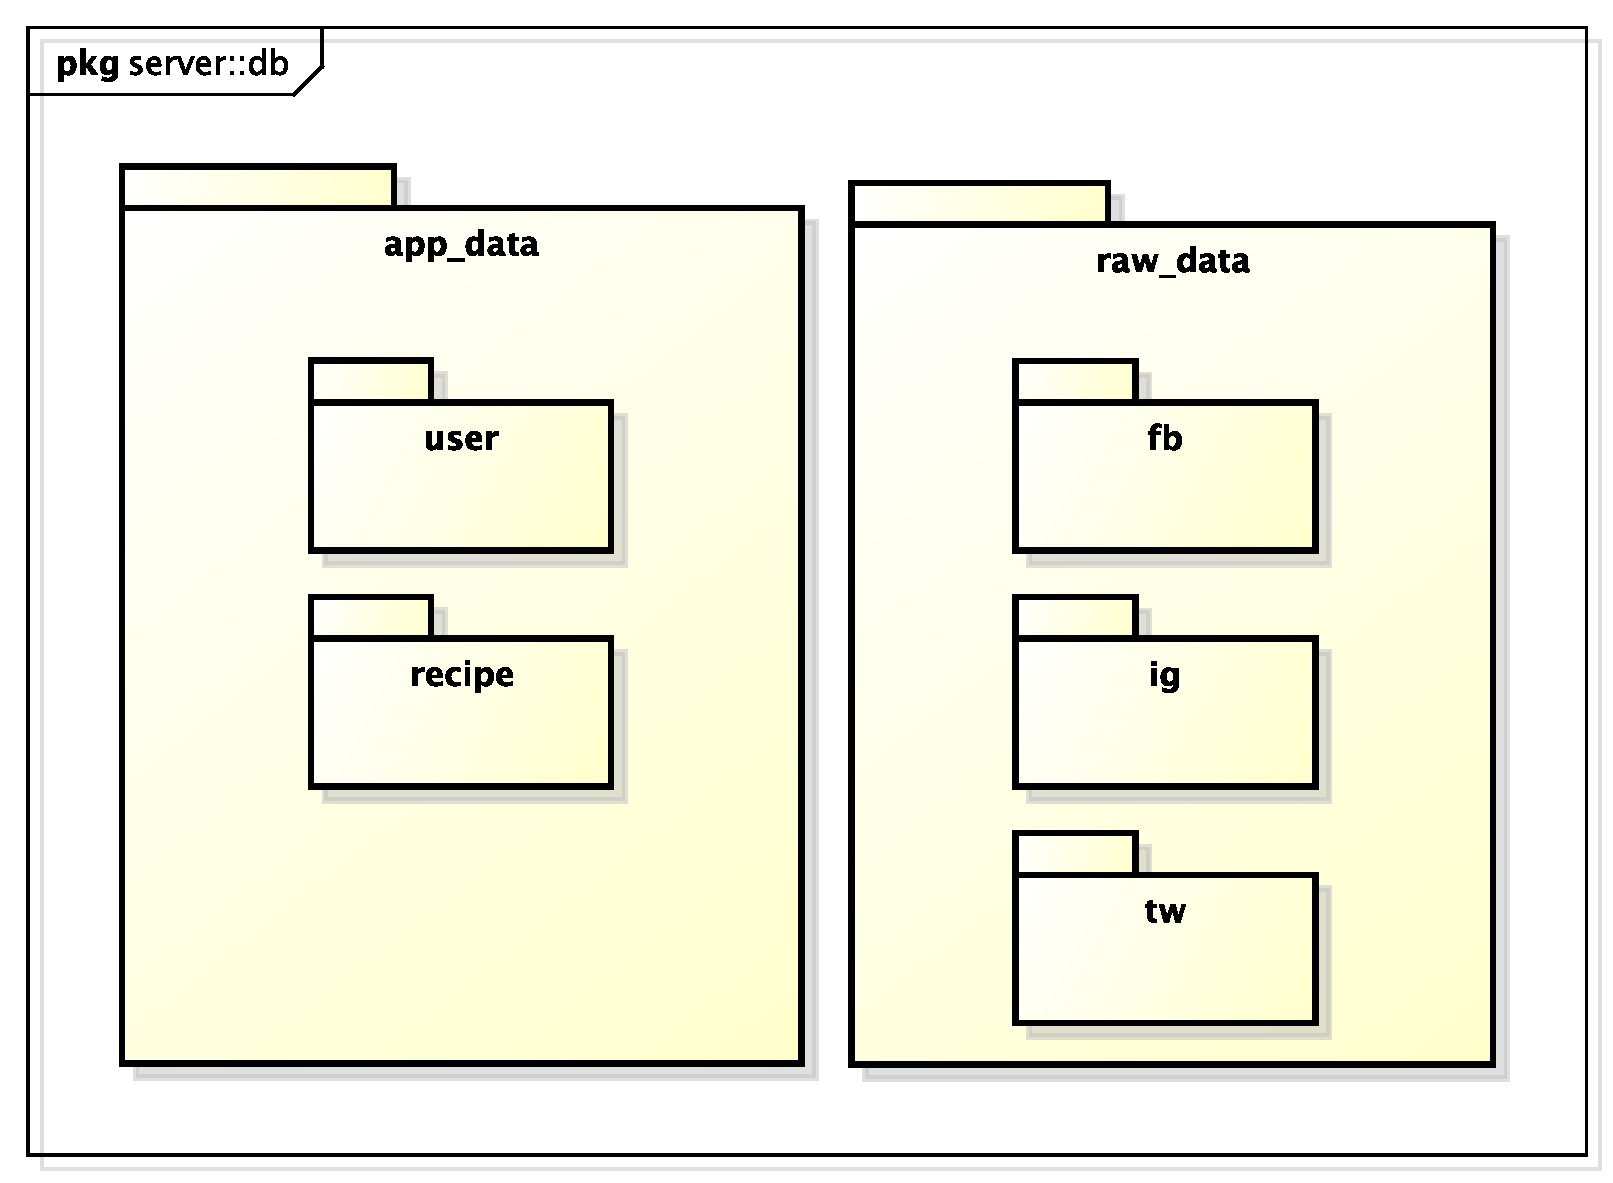
\includegraphics[scale=0.5]{./images/server/db.pdf}}
		\caption{Package - server::db}
	\end{figure}
	\begin{itemize}
		\item \textbf{Descrizione}: è il package che contiene le componenti che gestiscono e mantengono coerente la base di dati. Esse utilizzano standard proprietari Google per la loro implementazione. Sono suddivise in due package: uno atto a rappresentare il modello dei dati grezzi, l'altro per parametri del software e degli utenti;
		\item \textbf{Padre}: server;
		\item \textbf{Package contenuti}:
			\begin{itemize}
				\item server::app\_data.
				\item server::raw\_data;
			\end{itemize}
	\end{itemize}

% subsubsection RAW_DATA
\subsubsection{server::db::raw\_data} % (fold)
\label{ssub:bdsm_app_server_raw_data}
	\begin{figure}[htbp]
		\centering
		\centerline{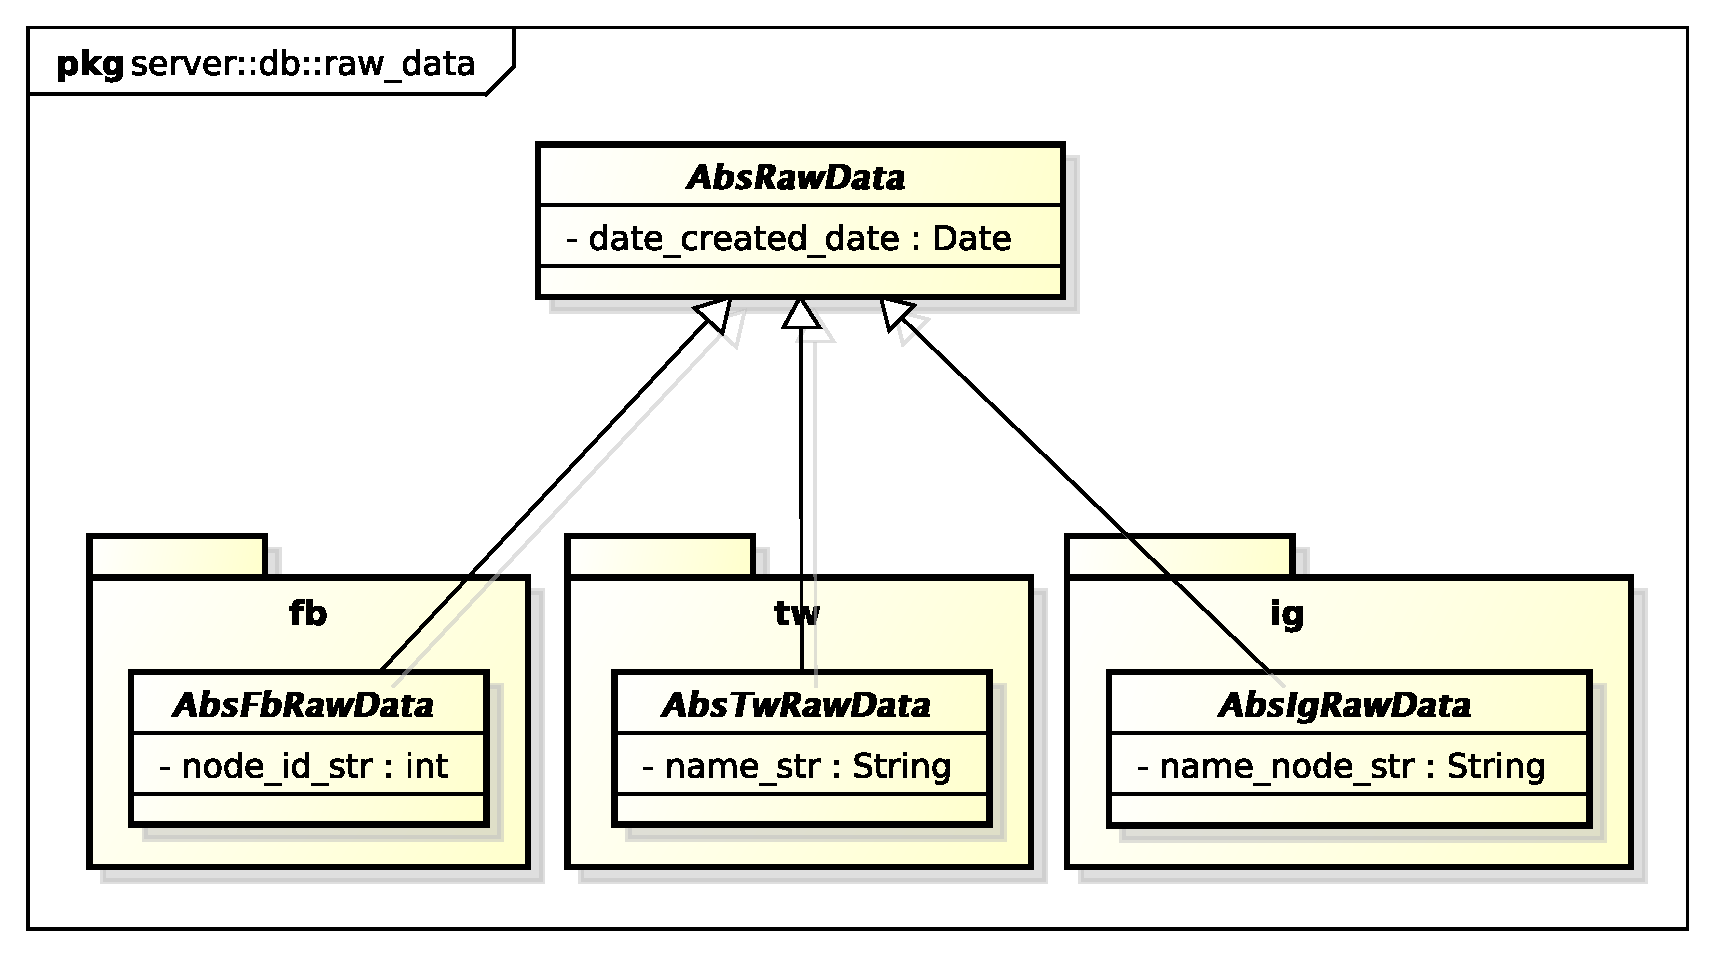
\includegraphics[scale=0.4]{./images/server/raw_data.pdf}}
		\caption{Package - server::db::raw\_data}
	\end{figure}
	\begin{itemize}
	\item \textbf{Descrizione}: package che definisce il modello dei dati grezzi ricavati dai vari social network;
		\item \textbf{Padre}: server::db;
		\item \textbf{Package contenuti}:
			\begin{itemize}
				\item server::db::raw\_data::fb
				\item server::db::raw\_data::tw
				\item server::db::raw\_data::ig
		\end{itemize}
	\end{itemize}

	\paragraph{Classi} % (fold)
		\subparagraph{server::db::raw\_data::AbsRawData} % (fold)
		\label{subp:bdsm_app_server_raw_data_absrawdata}
			\begin{itemize}
				\item \textbf{Descrizione}: classe astratta che definisce il modello di un dato grezzo;
				\item \textbf{Utilizzo}: la classe funge da padre per tutte le classi rappresentanti un dato grezzo;
				\item \textbf{Relazioni con altre classi}:
					\begin{itemize}
						\item server::db::raw\_data::fb::AbsFbRawData
						\item server::db::raw\_data::tw::AbsTwRawData
						\item server::db::raw\_data::ig::AbsIgRawData
						\item server::db::raw\_data::fb::RawFbPageTrend
						\item server::db::raw\_data::fb::RawFbEventTrend
						\item server::db::raw\_data::fb::RawFbPostTrendTrend
						\item server::db::raw\_data::tw::RawTwUserTrend
						\item server::db::raw\_data::tw::RawTwUserTweet
						\item server::db::raw\_data::ig::RawIgUserTrend
						\item server::db::raw\_data::ig::RawIgHashtagTrend
						\item server::db::raw\_data::ig::RawIgMedia
					\end{itemize}
				\item \textbf{Attributi}:
					\begin{itemize}
						\item \textcolor{forestgreen}{\texttt{+ date\_created\_date : Date}}
						\begin{description}
							\item \textbf{Descrizione}: data acquisizione dati grezzi
						\end{description}
					\end{itemize}
				\item \textbf{Metodi}: N/A
			\end{itemize}

		% subsubsection FACEBOOK
		\subsubsection{server::db::raw\_data::fb} % (fold)
		\label{ssub:bdsm_app_server_db_raw_data_fb}
		\begin{figure}[htbp]
			\centering
			\centerline{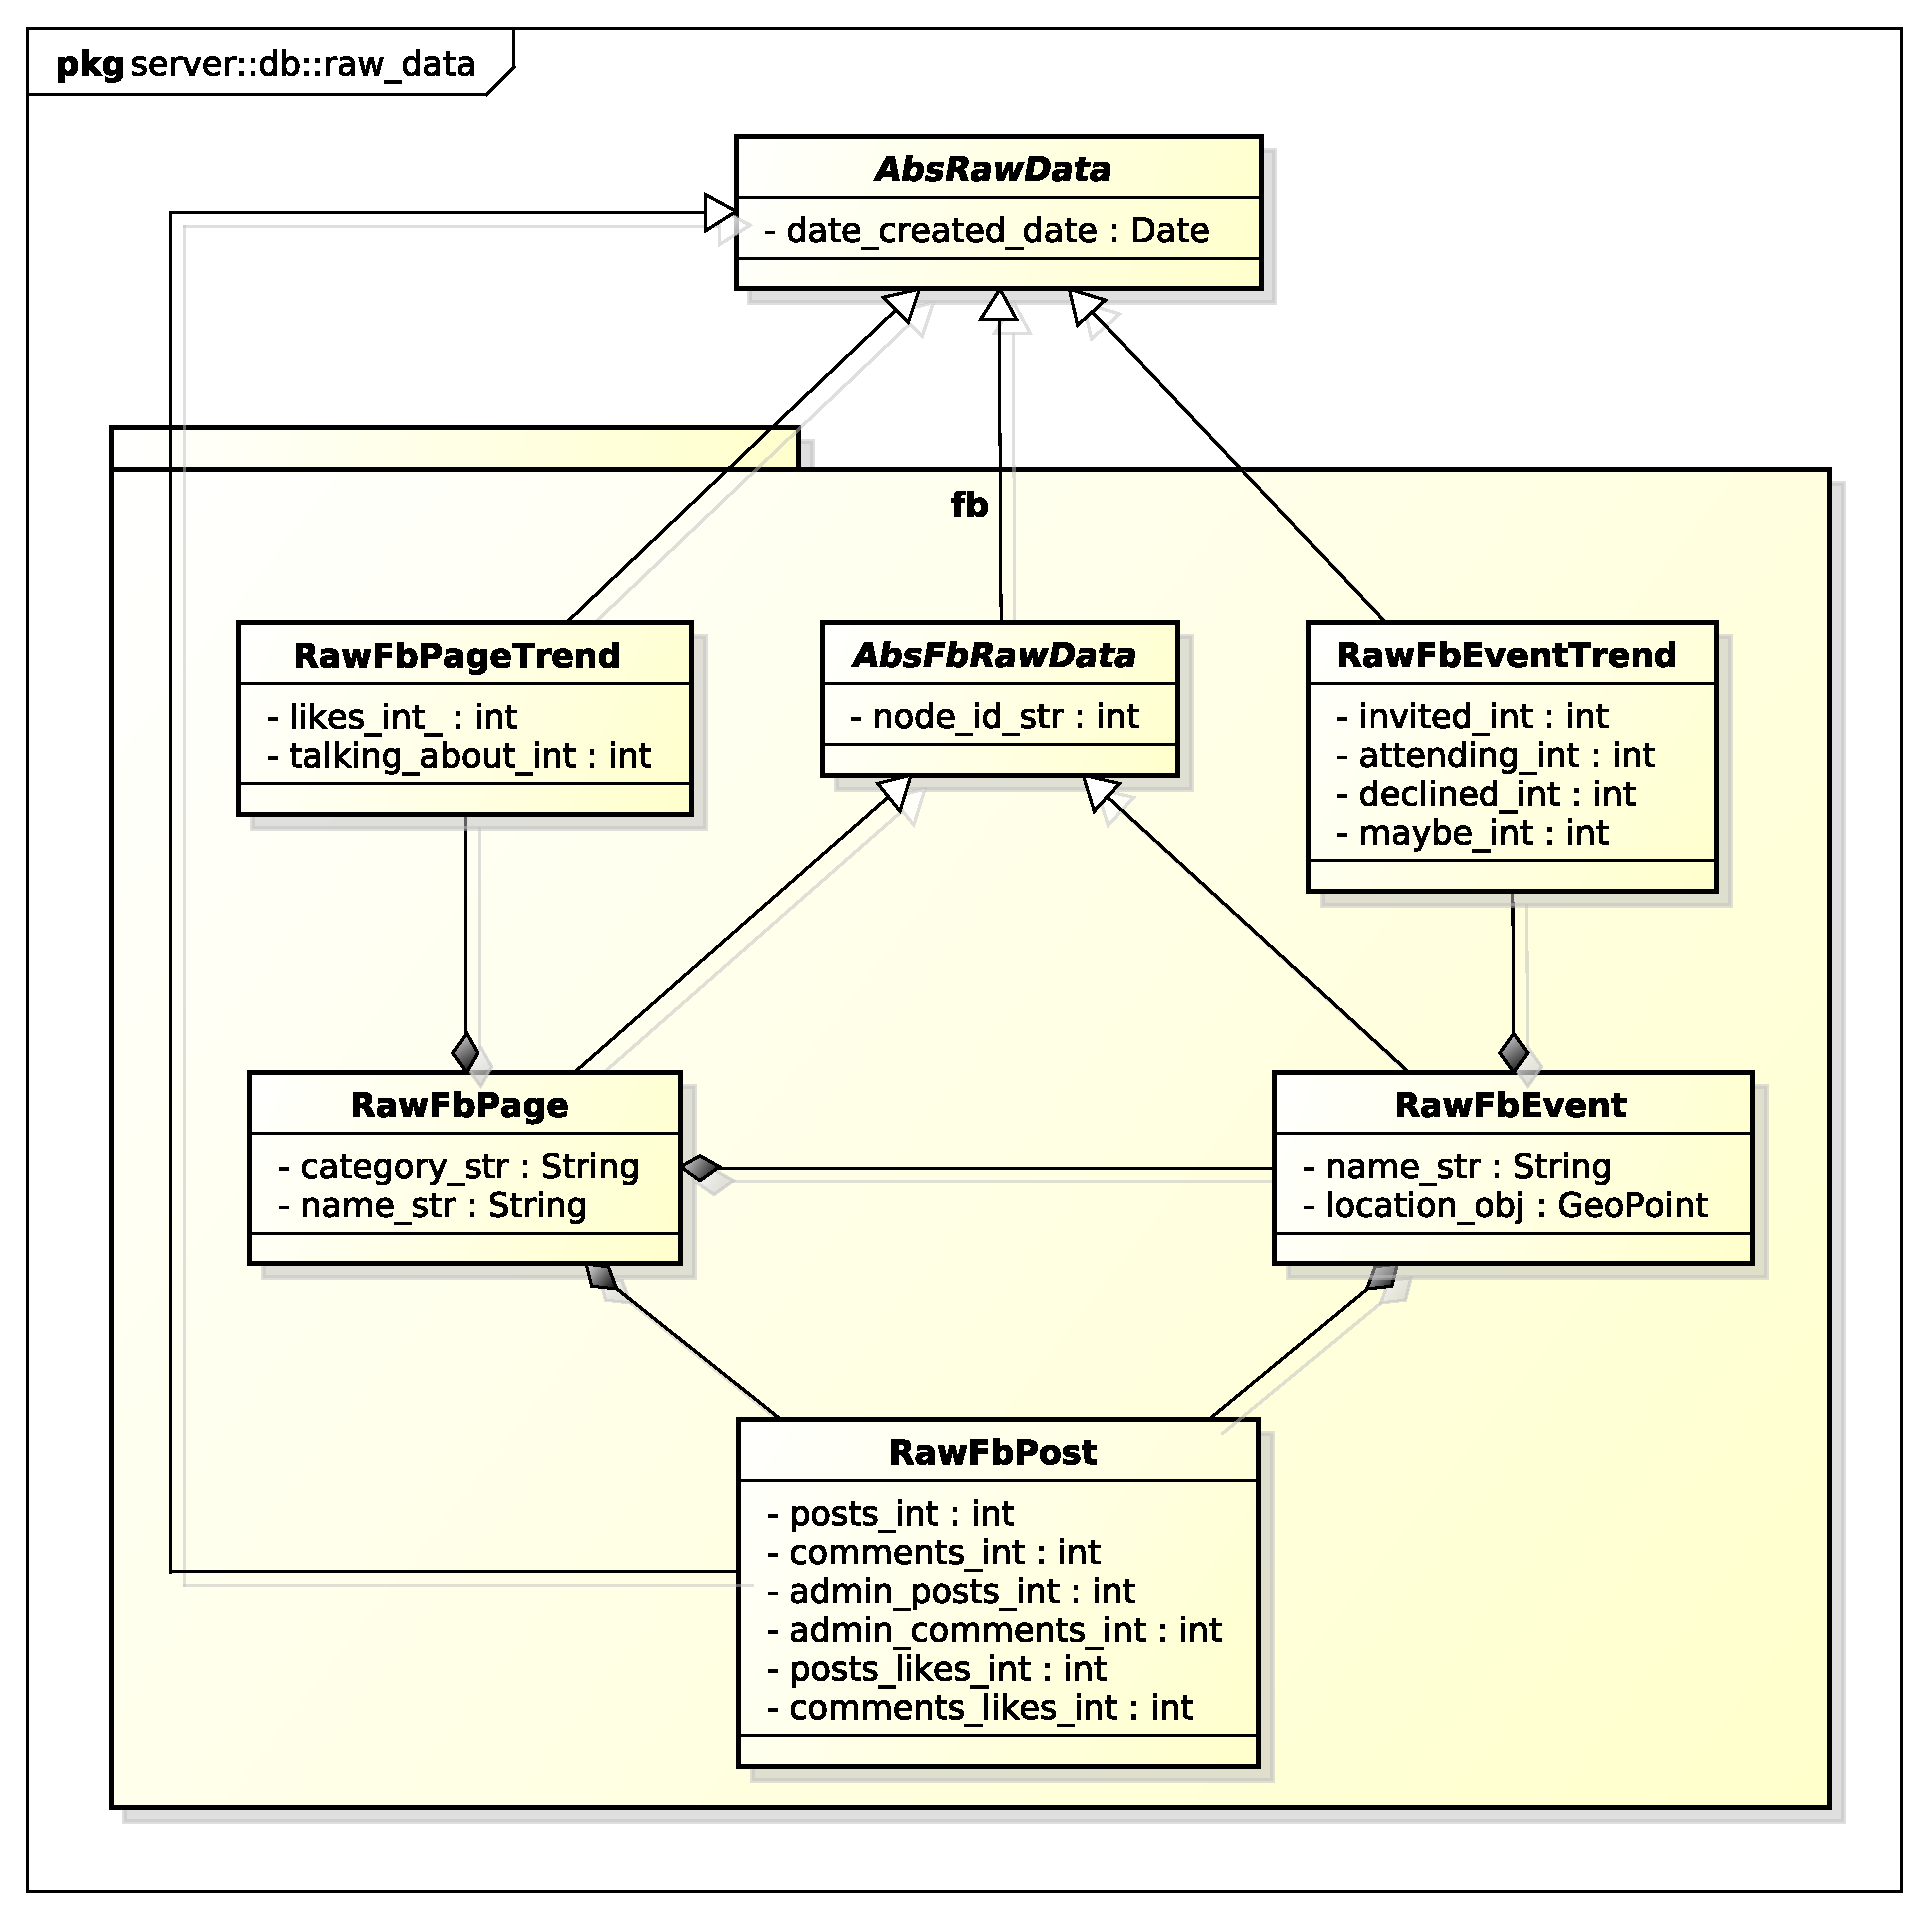
\includegraphics[scale=0.5]{./images/server/raw_data_fb.pdf}}
			\caption{Package - server::db::raw\_data::fb}
		\end{figure}
		\begin{itemize}
		  \item \textbf{Descrizione}:  è il package contenente le classi che definiscono i modelli dei dati grezzi relativi a Facebook;
		  \item \textbf{Padre}: server::db::raw\_data
		  \item \textbf{Interazione con altri componenti}:
		  	\begin{itemize}
		  		\item server::db
			\end{itemize}
		\end{itemize}
		% subsubsection

		\paragraph{Classi} % (fold)
			\subparagraph{server::db::raw\_data::fb::AbsFbRawData} % (fold)
			\label{subp:server_db_raw_data_fb_absfbrawdata}
				\begin{figure}[htbp]
					\centering
					\centerline{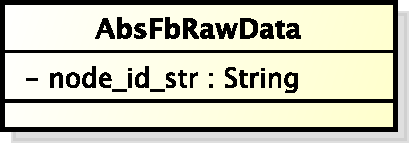
\includegraphics[scale=0.75]{./images/server/classes/db/abs_fb_raw_data.pdf}}
					\caption{Classe - server::db::raw\_data::fb::AbsFbRawData}
				\end{figure}
				\begin{itemize}
					\item \textbf{Descrizione}: classe astratta che definisce il modello dei dati grezzi relativi a Facebook;
					\item \textbf{Utilizzo}: la classe contiene l'id fornito dall'utente il quale permette di identificare univocamente la risorsa nel social media;
					\item \textbf{Classi ereditate}: server::db::raw\_data::AbsRawData
					\item \textbf{Attributi}:
					\begin{itemize}
						\item \textcolor{forestgreen}{\texttt{+ node\_id\_str : String}}
						\begin{description}
							\item \textbf{Descrizione}: codice identificativo di un evento o di una pagina Facebook.
						\end{description}
					\end{itemize}
					\item \textbf{Metodi}: N/A
				\end{itemize}
			% subparagraph server_db_raw_data_fb_absfbrawdata [end]


			\subparagraph{server::db::raw\_data::fb::RawFbPage} % (fold)
			\label{subp:server_db_raw_data_fb_rawfbpage}
				\begin{figure}[htbp]
					\centering
					\centerline{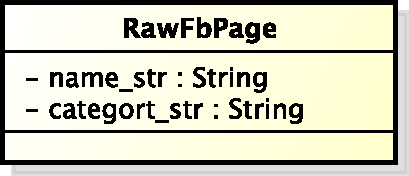
\includegraphics[scale=0.75]{./images/server/classes/db/raw_fb_page.pdf}}
					\caption{Classe - server::db::raw\_data::fb::RawFbPage}
				\end{figure}
				\begin{itemize}
					\item \textbf{Descrizione}: classe che rappresenta il modello di una pagina Facebook;
					\item \textbf{Utilizzo}: la classe fornisce metodi per memorizzare i dati statici di una pagina Facebook;
					\item \textbf{Classi ereditate}: server::db::raw\_data::AbsFbRawData
					\item \textbf{Relazioni con altre classi}:
						\begin{itemize}
							\item server::db::raw\_data::fb::RawFbEvent
							\item server::db::raw\_data::fb::RawFbPageTrend
							\item server::db::raw\_data::fb::RawFbPostTrend
						\end{itemize}
					\item \textbf{Attributi}:
					\begin{itemize}
						\item \textcolor{forestgreen}{\texttt{+ name\_str : String}}
						\begin{description}
							\item \textbf{Descrizione}: nome della pagina Facebook.
						\end{description}
						\item \textcolor{forestgreen}{\texttt{+ category\_str : String}}
						\begin{description}
							\item \textbf{Descrizione}: categoria della pagina Facebook.
						\end{description}
					\end{itemize}
					\item \textbf{Metodi}: N/A
				\end{itemize}
			% subparagraph server_db_raw_data_fb_rawfbpage [end]

			\subparagraph{server::db::raw\_data::fb::RawFbPageTrend} % (fold)
			\label{subp:server_db_raw_data_fb_rowfbpagetrend}
				\begin{figure}[htbp]
					\centering
					\centerline{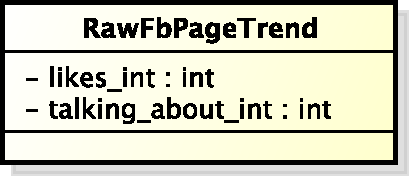
\includegraphics[scale=0.75]{./images/server/classes/db/raw_fb_page_trend.pdf}}
					\caption{Classe - server::db::raw\_data::fb::RawFbPageTrend}
				\end{figure}
				\begin{itemize}
					\item \textbf{Descrizione}: classe che rappresenta il modello del trend dei dati una pagina Facebook;
					\item \textbf{Utilizzo}: la classe viene utilizzata per memorizzare e il numero di like e di talking about di ogni singola pagina. Come per tutti gli oggetti di tipo trend, vengono ricavati i dati fino a 3 giorni prima della creazione dell'oggetto;
					\item \textbf{Classi ereditate}: server::db::raw\_data::AbsRawData
					\item \textbf{Attributi}:
					\begin{itemize}
						\item \textcolor{forestgreen}{\texttt{+ likes\_int : int}}
						\begin{description}
							\item \textbf{Descrizione}: numero dei likes di una determinata pagina Facebook,
						\end{description}
						\item \textcolor{forestgreen}{\texttt{+ talking\_about\_int : int}}
						\begin{description}
							\item \textbf{Descrizione}: numero di talking about di una determinata pagina Facebook.
						\end{description}
					\end{itemize}
					\item \textbf{Metodi}: N/A
				\end{itemize}
			% subparagraph server_db_raw_data_fb_rowfbpagetrend [end]


			\subparagraph{server::db::raw\_data::fb::RawFbEvent} % (fold)
			\label{subp:server_db_raw_data_fb_rawfbevent}
				\begin{figure}[htbp]
					\centering
					\centerline{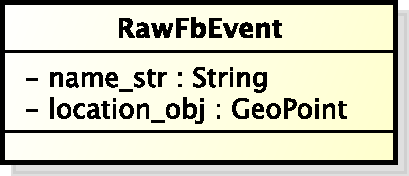
\includegraphics[scale=0.75]{./images/server/classes/db/raw_fb_event.pdf}}
					\caption{Classe - server::db::raw\_data::fb::RawFbEvent}
				\end{figure}
				\begin{itemize}
					\item \textbf{Descrizione}: classe che rappresenta il modello di un evento Facebook;
					\item \textbf{Utilizzo}: la classe fornisce metodi per memorizzare i dati statici di un evento Facebook;
					\item \textbf{Classi ereditate}: server::db::raw\_data::AbsFbRawData
					\item \textbf{Relazioni con altre classi}:
						\begin{itemize}
							\item server::db::raw\_data::fb::RawFbEventTrend
							\item server::db::raw\_data::fb::RawFbPostTrend
						\end{itemize}
					\item \textbf{Attributi}:
					\begin{itemize}
						\item \textcolor{forestgreen}{\texttt{+ name\_str : String}}
						\begin{description}
							\item \textbf{Descrizione}: nome dell'evento Facebook.
						\end{description}
						\item \textcolor{forestgreen}{\texttt{+ location\_obj : GeoPoint}}
						\begin{description}
							\item \textbf{Descrizione}: location dell'evento espressa in latitudine e longitudine.
						\end{description}
					\end{itemize}
					\item \textbf{Metodi}: N/A
				\end{itemize}
			% subparagraph server_db_raw_data_fb_rawfbevent [end]

			\subparagraph{server::db::raw\_data::fb::RawFbEventTrend} % (fold)
			\label{subp:server_db_raw_data_fb_rowfbeventtrend}
				\begin{figure}[htbp]
					\centering
					\centerline{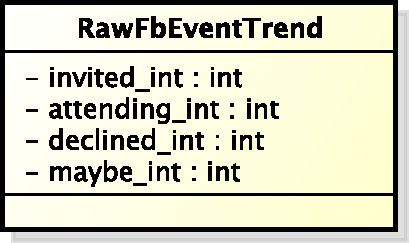
\includegraphics[scale=0.75]{./images/server/classes/db/raw_fb_event_trend.pdf}}
					\caption{Classe - server::db::raw\_data::fb::RawFbEventTrend}
				\end{figure}
				\begin{itemize}
					\item \textbf{Descrizione}: classe che rappresenta il modello del trend di un evento su Facebook;
					\item \textbf{Utilizzo}: la classe viene utilizzata per memorizzare il numero di utenti invitati, partecipanti e non di un evento. Come per tutti gli oggetti di tipo trend, vengono ricavati i dati fino a 3 giorni prima della creazione dell'oggetto;
					\item \textbf{Classi ereditate}: server::db::raw\_data::AbsRawData
					\item \textbf{Attributi}:
					\begin{itemize}
						\item \textcolor{forestgreen}{\texttt{+ invited\_int : int}}
						\begin{description}
							\item \textbf{Descrizione}: numero delle persone invitate all'evento Facebook.
						\end{description}
						\item \textcolor{forestgreen}{\texttt{+ attending\_int : int}}
						\begin{description}
							\item \textbf{Descrizione}: numero persone partecipanti all'evento Facebook
						\end{description}
						\item \textcolor{forestgreen}{\texttt{+ declined\_int : int}}
						\begin{description}
							\item \textbf{Descrizione}: numero persone che hanno rifiutato la partecipazione all'evento Facebook.
						\end{description}
						\item \textcolor{forestgreen}{\texttt{+ maybe\_int : int}}
						\begin{description}
							\item \textbf{Descrizione}: numero persone incerte se partecipare all'evento Facebook.
						\end{description}
					\end{itemize}
					\item \textbf{Metodi}: N/A
				\end{itemize}
			% subparagraph server_db_raw_data_fb_rowfbeventtrend [end]


			\subparagraph{server::db::raw\_data::fb::RawFbPostTrend} % (fold)
			\label{subp:server_db_raw_data_fb_RawFbPostTrend}
				\begin{figure}[htbp]
					\centering
					\centerline{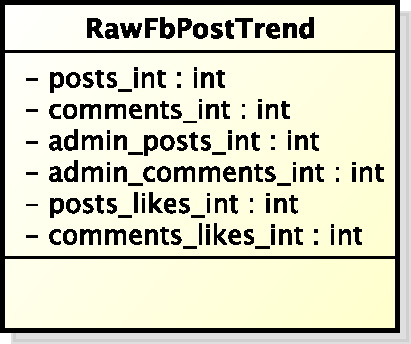
\includegraphics[scale=0.75]{./images/server/classes/db/raw_fb_post_trend.pdf}}
					\caption{Classe - server::db::raw\_data::fb::RawFbPostTrend}
				\end{figure}
				\begin{itemize}
					\item \textbf{Descrizione}: classe che rappresenta il modello del trend dei post di una pagina o di un evento su Facebook;
					\item \textbf{Utilizzo}: viene utilizzata per memorizzare i dati relativi al trend dei post di una pagina o un pagina o evento Facebook. Come per tutti gli oggetti di tipo trend, vengono ricavati i dati fino a 3 giorni prima della creazione dell'oggetto;
					\item \textbf{Attributi}:
					\begin{itemize}
						\item \textcolor{forestgreen}{\texttt{+ posts\_int : int}}
						\begin{description}
							\item \textbf{Descrizione}: numero dei post presenti nella pagina o nell'evento.
						\end{description}
						\item \textcolor{forestgreen}{\texttt{+ comments\_int : int}}
						\begin{description}
							\item \textbf{Descrizione}: numero totale di commenti ai post della pagina o dell'evento.
						\end{description}
						\item \textcolor{forestgreen}{\texttt{+ admin\_posts\_int : int}}
						\begin{description}
							\item \textbf{Descrizione}: numero dei post effettuati esclusivamente da una pagina Facebook e non da terzi.
						\end{description}
						\item \textcolor{forestgreen}{\texttt{+ admin\_comments\_int : int}}
						\begin{description}
							\item \textbf{Descrizione}: numero dei commenti effettuati esclusivamente da una pagina Facebook e non da terzi.
						\end{description}
						\item \textcolor{forestgreen}{\texttt{+ posts\_like\_int : int}}
						\begin{description}
							\item \textbf{Descrizione}: numero totale dei likes ai post di una pagina o evento Facebook.
						\end{description}
						\item \textcolor{forestgreen}{\texttt{+ comments\_like\_int : int}}
						\begin{description}
							\item \textbf{Descrizione}: numero totale ai likes dei commenti presenti nei post di una pagina o evento Facebook.
						\end{description}
					\end{itemize}
					\item \textbf{Metodi}: N/A
				\end{itemize}
			% subparagraph server_db_raw_data_fb_RawFbPostTrend [end]


		% subsubsection TWITTER
		\subsubsection{server::db::raw\_data::tw} % (fold)
		\label{ssub:bdsm_app_server_db_raw_data_tw}
		\begin{figure}[htbp]
			\centering
			\centerline{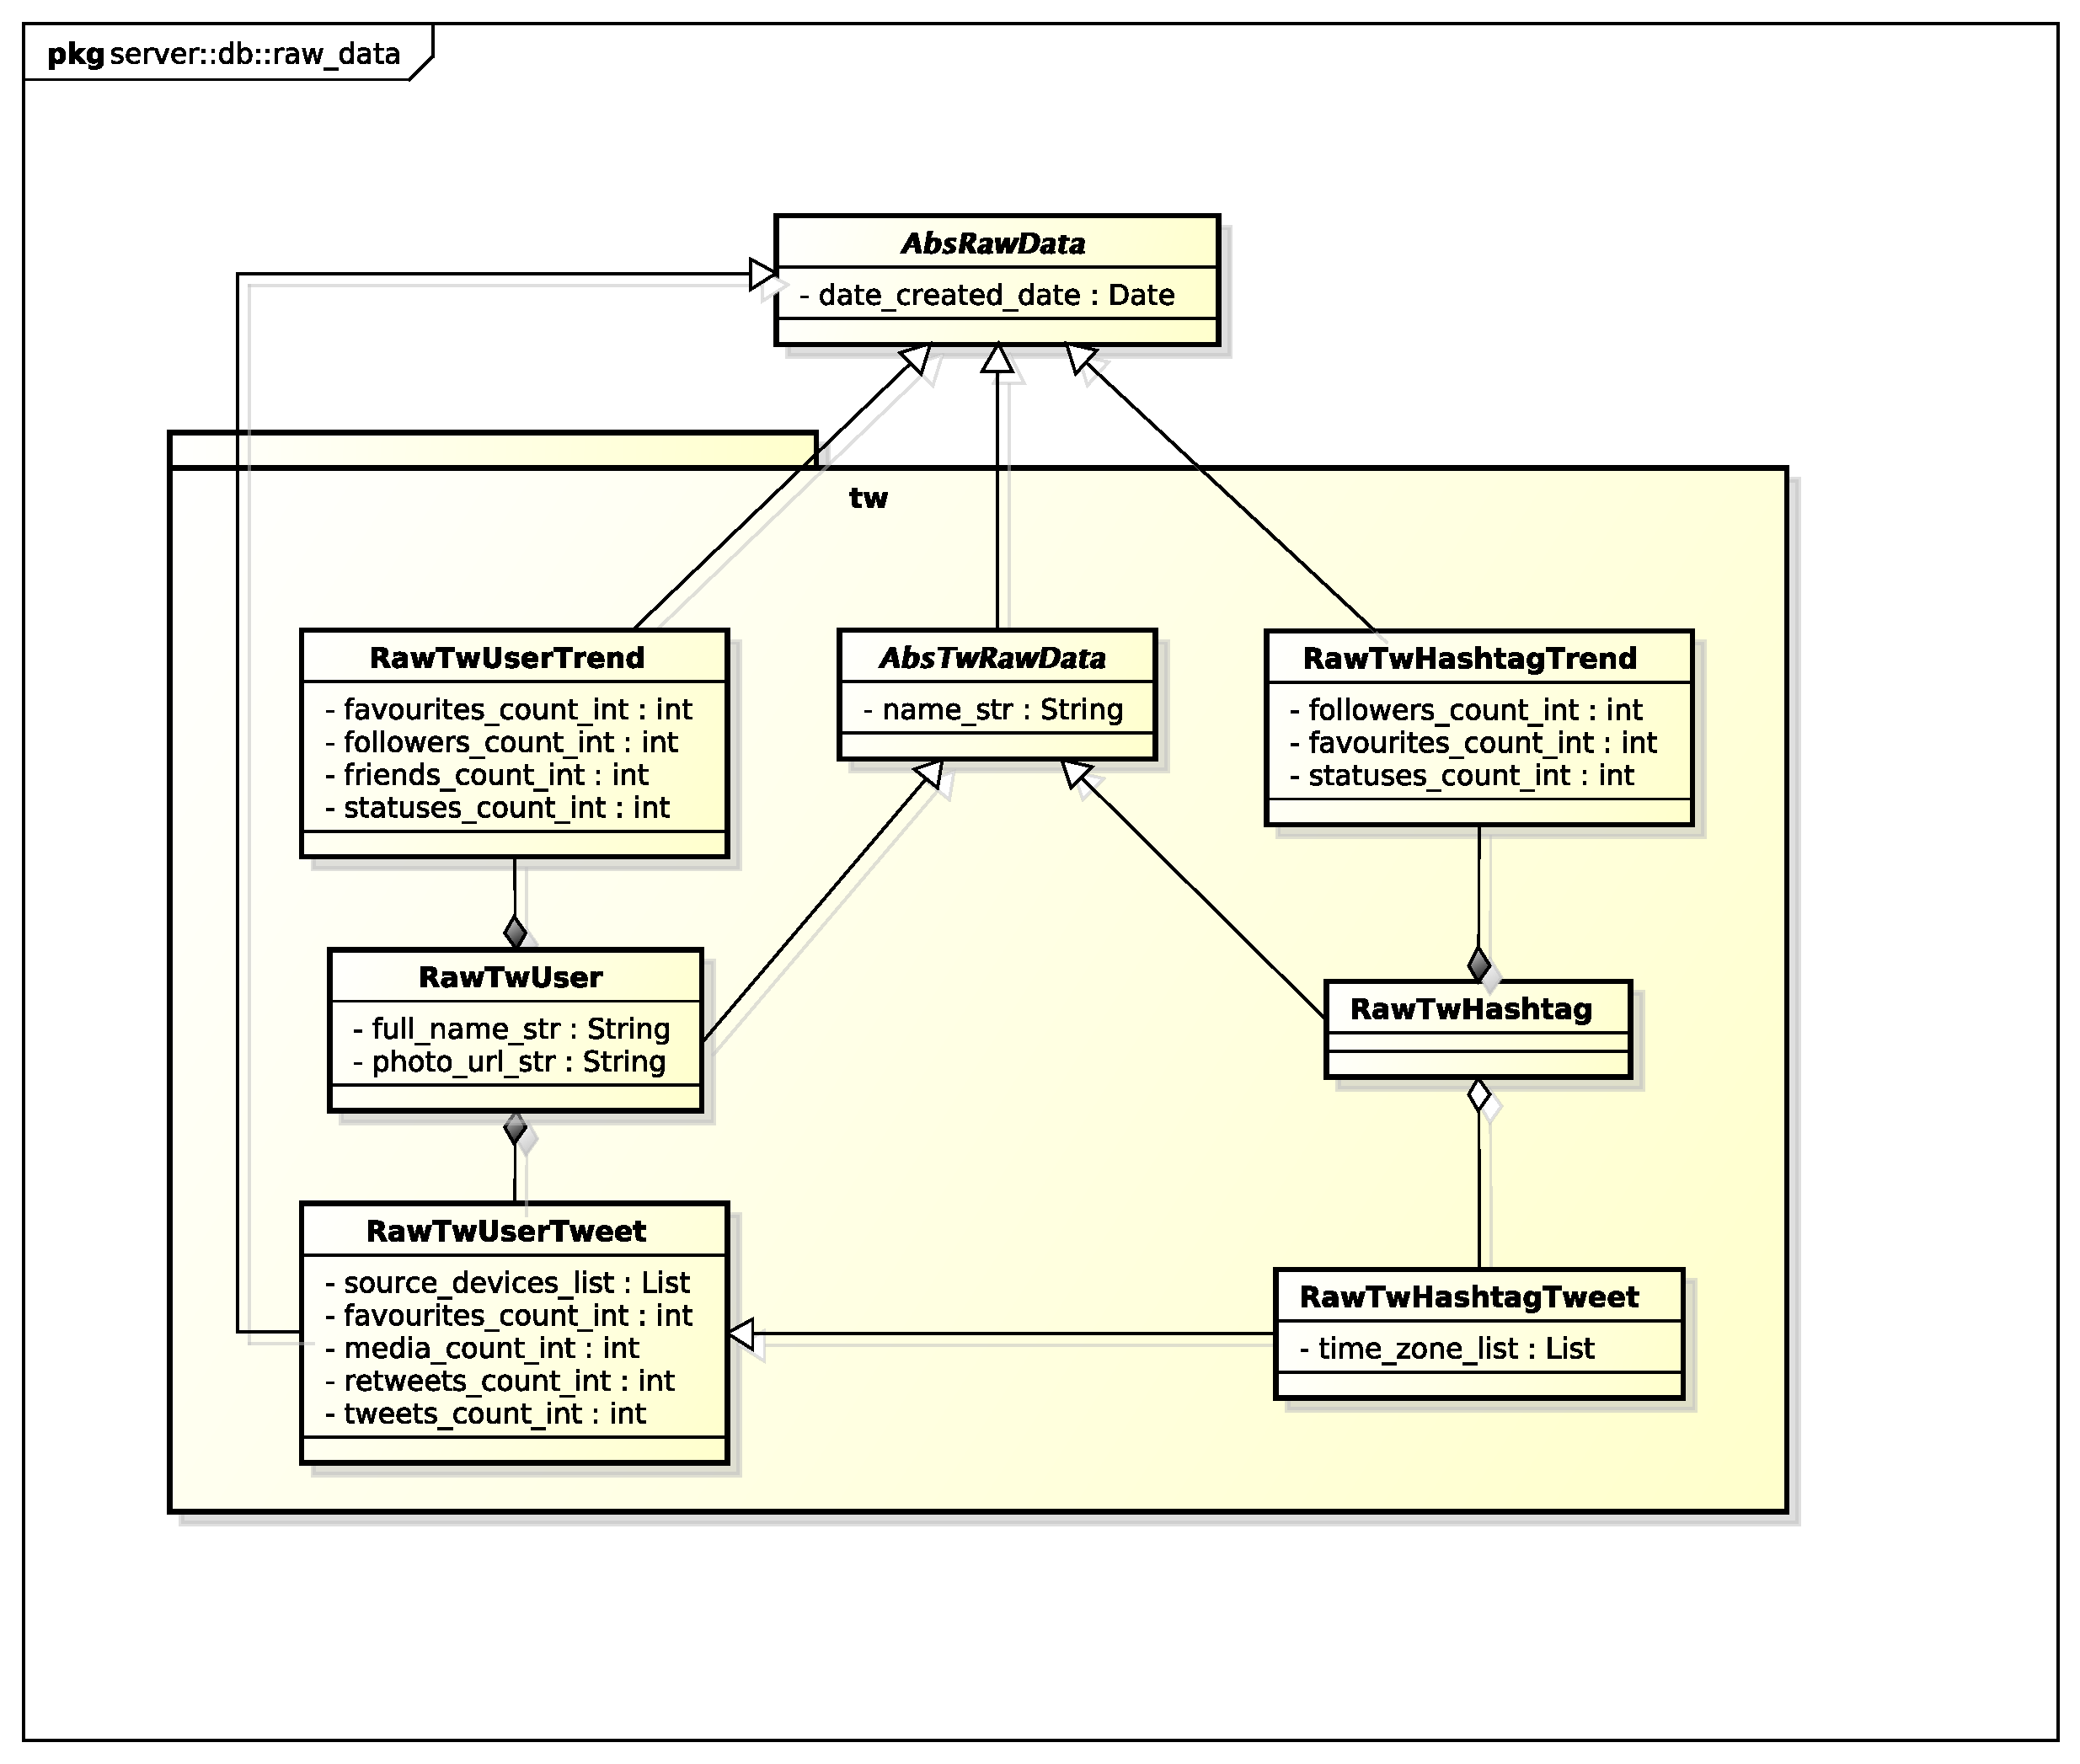
\includegraphics[scale=0.45]{./images/server/raw_data_tw.pdf}}
			\caption{Package - server::db::raw\_data::tw}
		\end{figure}

		\begin{itemize}
		  \item \textbf{Descrizione}: è il package contenente le classi che definiscono i modelli dei dati grezzi relativi a Twitter;
		  \item \textbf{Padre}: server::db::raw\_data
		  \item \textbf{Interazione con altri componenti}:
		  	\begin{itemize}
		  		\item server::db
			\end{itemize}
		\end{itemize}
		% subsubsection

		\paragraph{Classi} % (fold)


		\subparagraph{server::db::raw\_data::tw::AbsTwRawData} % (fold)
		\label{subp:server_db_raw_data_tw_abstwrawdata}
			\begin{figure}[htbp]
				\centering
				\centerline{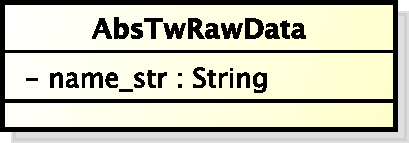
\includegraphics[scale=0.75]{./images/server/classes/db/abs_tw_raw_data.pdf}}
				\caption{Classe - server::db::raw\_data::tw::AbsTwRawData}
			\end{figure}
			\begin{itemize}
				\item \textbf{Descrizione}: classe astratta che definisce il modello dei dati grezzi relativi a Twitter;
				\item \textbf{Utilizzo}: la classe contiene l'id fornito dall'utente il quale permette di identificare univocamente la risorsa nel social media;
				\item \textbf{Classi ereditate}: server::db::raw\_data::AbsRawData
				\item \textbf{Attributi}:
					\begin{itemize}
						\item \textcolor{forestgreen}{\texttt{+ name\_str : String}}
						\begin{description}
							\item \textbf{Descrizione}: nome identificativo della pagina o dell'hashtag Twitter.
						\end{description}
					\end{itemize}
				\item \textbf{Metodi}: N/A
			\end{itemize}
		% subparagraph server_db_raw_data_tw_abstwrawdata [end]


		\subparagraph{server::db::raw\_data::tw::RawTwUser} % (fold)
		\label{subp:server_db_raw_data_tw_rawtwuser}
			\begin{figure}[htbp]
				\centering
				\centerline{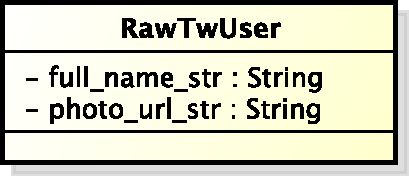
\includegraphics[scale=0.75]{./images/server/classes/db/raw_tw_user.pdf}}
				\caption{Classe - server::db::raw\_data::tw::RawTwUser}
			\end{figure}
			\begin{itemize}
				\item \textbf{Descrizione}: classe che definisce il modello dei dati di un utente Twitter;
				\item \textbf{Utilizzo}: la classe viene utilizzata per fornire una descrizione completa dell'utente Twitter. Vengono forniti metodi automatici per il conteggio dei parametri che verranno utilizzati per seguire un trend;;
				\item \textbf{Classi ereditate}: server::db::raw\_data::AbsTwRawData
				\item \textbf{Relazioni con altre classi}:
					\begin{itemize}
						\item server::db::raw\_data::tw::RawTwUserTrend
						\item server::db::raw\_data::tw::RawTwUserTweet
					\end{itemize}
				\item \textbf{Attributi}:
					\begin{itemize}
						\item \textcolor{forestgreen}{\texttt{+ full\_name\_str : String}}
						\begin{description}
							\item \textbf{Descrizione}: nome completo dell'utente Twitter.
						\end{description}
						\item \textcolor{forestgreen}{\texttt{+ photo\_url\_str : String}}
						\begin{description}
							\item \textbf{Descrizione}: indirizzo url della foto profilo dell'utente Twitter.
						\end{description}
					\end{itemize}
				\item \textbf{Metodi}: N/A
			\end{itemize}
		% subparagraph server_db_raw_data_tw_rawtwuser [end]


		\subparagraph{server::db::raw\_data::tw::RawTwUserTrend} % (fold)
		\label{subp:server_db_raw_data_tw_rawtwusertrend}
			\begin{figure}[htbp]
				\centering
				\centerline{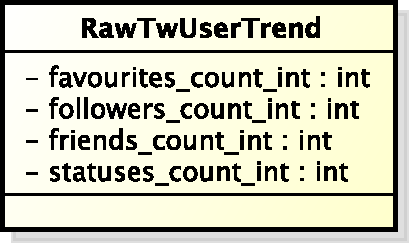
\includegraphics[scale=0.75]{./images/server/classes/db/raw_tw_user_trend.pdf}}
				\caption{Classe - server::db::raw\_data::tw::RawTwUserTrend}
			\end{figure}
			\begin{itemize}
				\item \textbf{Descrizione}: classe che definisce il modello dei dati del trend di un utente Twitter;
				\item \textbf{Utilizzo}: la classe viene utilizzata per memorizzare il numero di favoriti, di followers, di friends e statuses di un determinato utente Twitter. Come per tutti gli oggetti di tipo trend, vengono ricavati i dati fino a 3 giorni prima della creazione dell'oggetto;
				\item \textbf{Classi ereditate}: server::db::raw\_data::AbsTwRawData
				\item \textbf{Attributi}:
					\begin{itemize}
						\item \textcolor{forestgreen}{\texttt{+ favourites\_count\_int : int}}
						\begin{description}
							\item \textbf{Descrizione}: numero totale dei preferiti assegnati dall'utente.
						\end{description}
						\item \textcolor{forestgreen}{\texttt{+ followers\_count\_int : int}}
						\begin{description}
							\item \textbf{Descrizione}: numero dei followers di un utente Twitter.
						\end{description}
						\item \textcolor{forestgreen}{\texttt{+ friends\_count\_int : int}}
						\begin{description}
							\item \textbf{Descrizione}: numero dei following di un utente Twitter.
						\end{description}
						\item \textcolor{forestgreen}{\texttt{+ tweets\_count\_int : int}}
						\begin{description}
							\item \textbf{Descrizione}: numero di tweets di un utente Twitter.
						\end{description}
					\end{itemize}
				\item \textbf{Metodi}: N/A
			\end{itemize}
		% subparagraph server_db_raw_data_tw_rawigusertrend [end]


		\subparagraph{server::db::raw\_data::tw::RawTwUserTweet} % (fold)
		\label{subp:server_db_raw_data_tw_rawtwusertweet}
			\begin{figure}[htbp]
				\centering
				\centerline{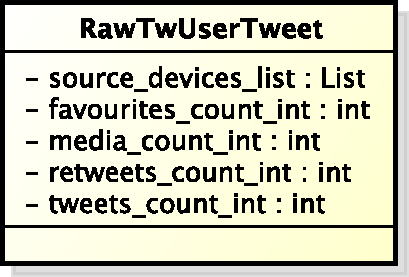
\includegraphics[scale=0.75]{./images/server/classes/db/raw_tw_user_tweet.pdf}}
				\caption{Classe - server::db::raw\_data::tw::RawTwUserTweet}
			\end{figure}
			\begin{itemize}
				\item \textbf{Descrizione}: classe che definisce il modello dei dati del trend dei tweet relativi ad un utente Twitter;
				\item \textbf{Utilizzo}: la classe viene utilizzata per fornire una descrizione dettagliata di un tweet creato da un utente specifico su Twitter;
				\item \textbf{Classi ereditate}: server::db::raw\_data::AbsRawData
				\item \textbf{Attributi}:
					\begin{itemize}
						\item \textcolor{forestgreen}{\texttt{+ source\_devices\_list : List}}
						\begin{description}
							\item \textbf{Descrizione}: lista composta da quantità e tipo dispositivi utilizzati in relazione ai tweet di un utente Twitter.
						\end{description}
						\item \textcolor{forestgreen}{\texttt{+ favourites\_count\_int : int}}
						\begin{description}
							\item \textbf{Descrizione}: totale dei preferiti aggiunti ai tweet di un utente.
						\end{description}
						\item \textcolor{forestgreen}{\texttt{+ retweets\_count\_int : int}}
						\begin{description}
							\item \textbf{Descrizione}: numero totale dei retweet ai tweets di utente Twitter.
						\end{description}
					\end{itemize}
				\item \textbf{Metodi}: N/A
			\end{itemize}
		% subparagraph server_db_raw_data_tw_rawtwusertweet [end]


		\subparagraph{server::db::raw\_data::tw::RawTwHashtag} % (fold)
		\label{subp:server_db_raw_data_tw_rawtwhashtag}
			\begin{itemize}
				\item \textbf{Descrizione}: classe che definisce il modello dei dati di un hashtag su Twitter;
				\item \textbf{Utilizzo}: la classe viene utilizzata per fornire una descrizione minimale di un hashtag su Twitter. Sebbene tale classe non presenti metodi o attributi, risulta molto utile per distinguere un hashtag Twitter da un'altra metrica effettuando un type checking;
				\item \textbf{Classi ereditate}: server::db::raw\_data::AbsTwRawData
				\item \textbf{Relazioni con altre classi}:
					\begin{itemize}
						\item server::db::raw\_data::tw::RawTwHashtagTweet
					\end{itemize}
				\item \textbf{Attributi}: N/A
				\item \textbf{Metodi}: N/A
			\end{itemize}
		% subparagraph server_db_raw_data_tw_rawtwhashtag [end]


		\subparagraph{server::db::raw\_data::tw::RawTwHashtagTweet} % (fold)
		\label{subp:server_db_raw_data_tw_rawtwhashtagtweet}
			\begin{figure}[htbp]
				\centering
				\centerline{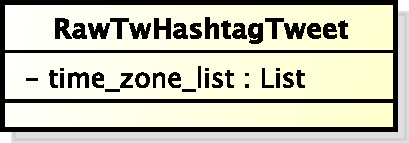
\includegraphics[scale=0.75]{./images/server/classes/db/raw_tw_hashtag_tweet.pdf}}
				\caption{Classe - server::db::raw\_data::tw::RawTwHashtagTweet}
			\end{figure}
			\begin{itemize}
				\item \textbf{Descrizione}: classe che definisce il modello dei dati del trend dei tweet relativi ad un hashtag Twitter;
				\item \textbf{Utilizzo}: la classe viene utilizzata per fornire una descrizione della locazione spaziale di un tweet relativo all'hashtag su Twitter. Come per tutti gli oggetti di tipo trend, vengono ricavati i dati fino a 3 giorni prima della creazione dell'oggetto;
				\item \textbf{Classi ereditate}: server::db::raw\_data::RawTwUserTweet
				\item \textbf{Attributi}:
					\begin{itemize}
						\item \textcolor{forestgreen}{\texttt{+ time\_zone\_list : List}}
						\begin{description}
							\item \textbf{Descrizione}: contiene informazioni sulle timezone ricavate dai vari tweet contenenti un determinato hashtag Twitter e dalle occorrenze delle stesse.
						\end{description}
						\item \textcolor{forestgreen}{\texttt{+ tweets\_count\_int : int}}
						\begin{description}
							\item \textbf{Descrizione}: totale dei tweet contenenti un determinato hashtag.
						\end{description}
					\end{itemize}
				\item \textbf{Metodi}: N/A
			\end{itemize}
		% subparagraph server_db_raw_data_tw_rawtwhashtagtweet [end]


		% subsubsection INSTAGRAM
		\subsubsection{server::db::raw\_data::ig} % (fold)
		\label{ssub:bdsm_app_server_db_raw_data_ig}
		\begin{figure}[htbp]
			\centering
			\centerline{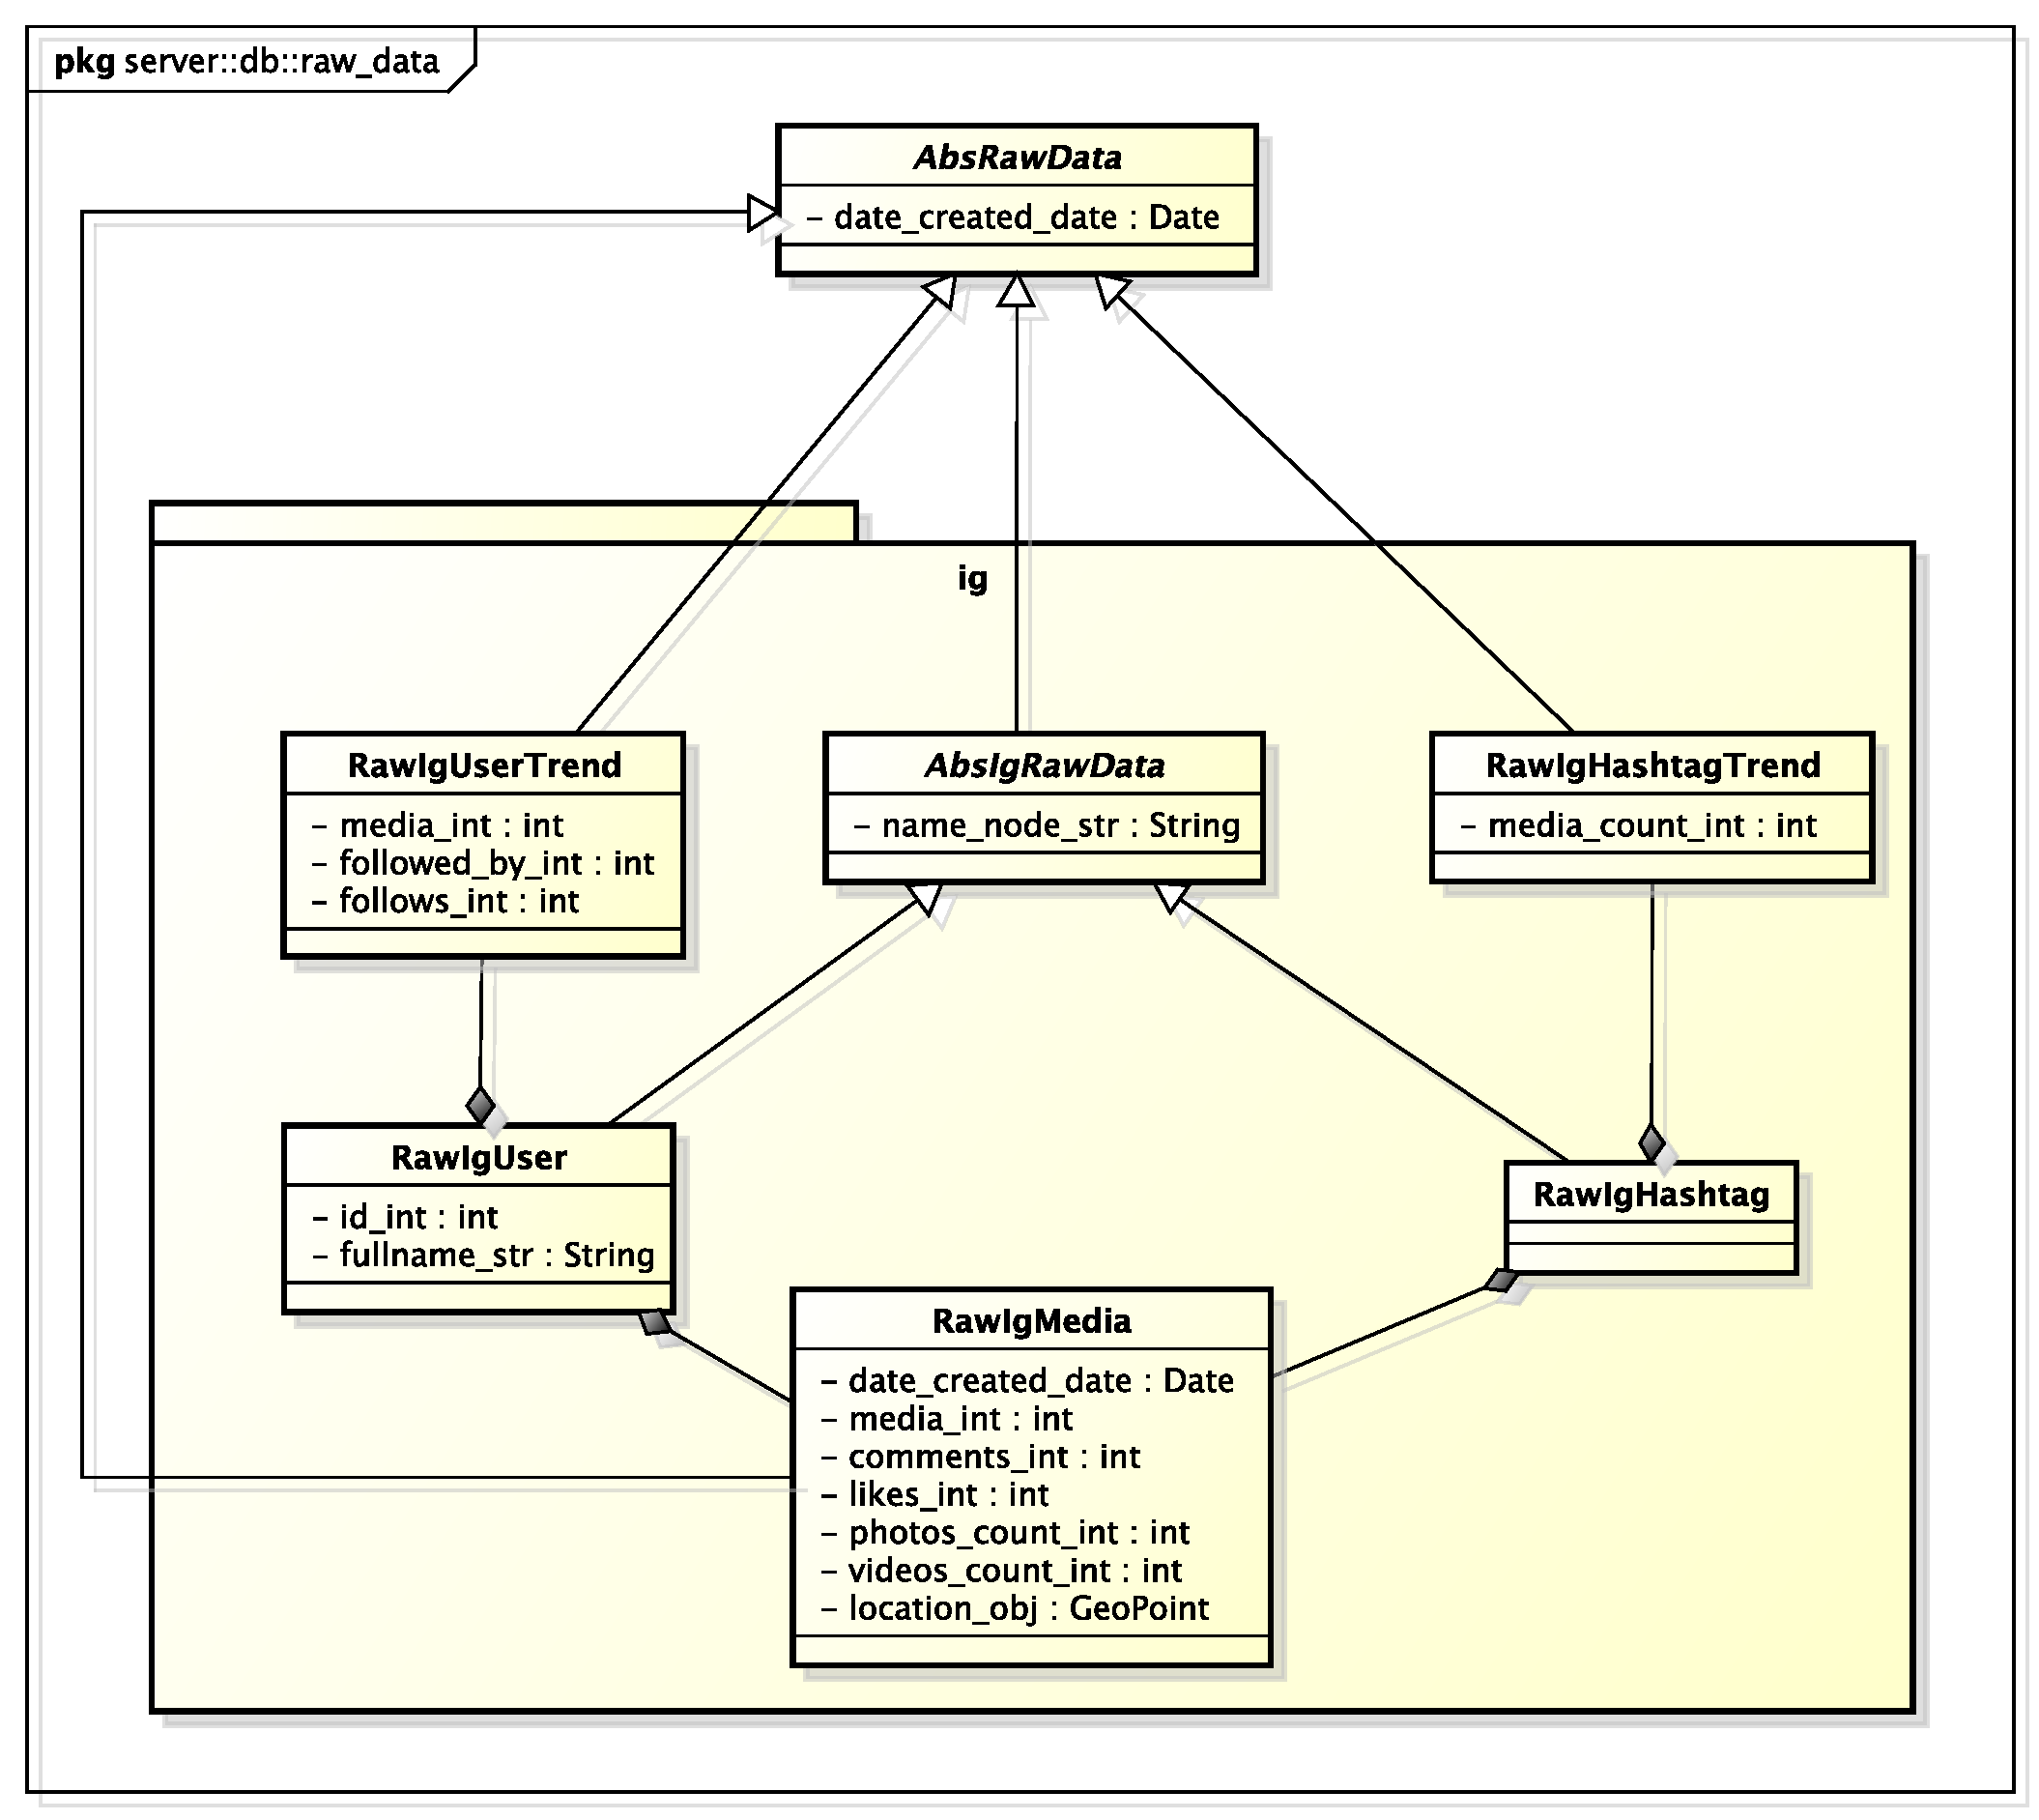
\includegraphics[scale=0.5]{./images/server/raw_data_ig.pdf}}
			\caption{Package - server::db::raw\_data::ig}
		\end{figure}

		\begin{itemize}
		  \item \textbf{Descrizione}: è il package contenente le classi che definiscono i modelli dei dati grezzi relativi a Instagram;
		  \item \textbf{Padre}: server::db::raw\_data
		  \item \textbf{Interazione con altri componenti}:
		  	\begin{itemize}
		  		\item server::db
				\end{itemize}
		\end{itemize}
		% subsubsection

		\paragraph{Classi} % (fold)


		\subparagraph{server::db::raw\_data::ig::AbsIgRawData} % (fold)
		\label{subp:server_db_raw_data_ig_absigrawdata}
			\begin{figure}[htbp]
				\centering
				\centerline{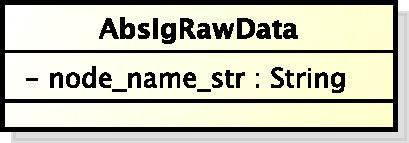
\includegraphics[scale=0.75]{./images/server/classes/db/abs_ig_raw_data.pdf}}
				\caption{Classe - server::db::raw\_data::ig::AbsIgRawData}
			\end{figure}
			\begin{itemize}
				\item \textbf{Descrizione}: classe astratta che definisce il modello dei dati grezzi relativi ad Instagram;
				\item \textbf{Utilizzo}: la classe contiene l'id fornito dall'utente il quale permette di identificare univocamente la risorsa nel social media;
				\item \textbf{Classi ereditate}: server::db::raw\_data::AbsRawData
				\item \textbf{Attributi}:
					\begin{itemize}
						\item \textcolor{forestgreen}{\texttt{+ node\_name\_str : String}}
						\begin{description}
							\item \textbf{Descrizione}: nome identificativo di un utente o di un hashtag Instagram.
						\end{description}
					\end{itemize}
				\item \textbf{Metodi}: N/A
			\end{itemize}
		% subparagraph server_db_raw_data_ig_absigrawdata [end]


		\subparagraph{server::db::raw\_data::ig::RawIgUser} % (fold)
		\label{subp:server_db_raw_data_ig_rawiguser}
			\begin{figure}[htbp]
				\centering
				\centerline{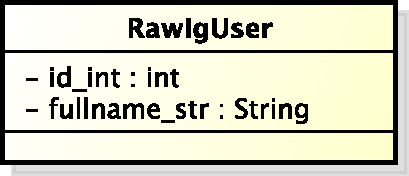
\includegraphics[scale=0.75]{./images/server/classes/db/raw_ig_user.pdf}}
				\caption{Classe - server::db::raw\_data::ig::RawIgUser}
			\end{figure}
			\begin{itemize}
				\item \textbf{Descrizione}: classe che definisce il modello dei dati di un utente Instagram;
				\item \textbf{Utilizzo}:  la classe viene utilizzata per memorizzare i dettagli di un utente Instagram;
				\item \textbf{Classi ereditate}: server::db::raw\_data::AbsIgRawData
				\item \textbf{Relazioni con altre classi}:
					\begin{itemize}
						\item server::db::raw\_data::ig::RawIgUserTrend
						\item server::db::raw\_data::ig::RawIgMedia
					\end{itemize}
				\item \textbf{Attributi}:
					\begin{itemize}
						\item \textcolor{forestgreen}{\texttt{+ id\_int : int}}
						\begin{description}
							\item \textbf{Descrizione}: numero identificativo di utente Instagram.
						\end{description}
						\item \textcolor{forestgreen}{\texttt{+ fullname\_str : String}}
						\begin{description}
							\item \textbf{Descrizione}: nome completo di utente Instagram.
						\end{description}
					\end{itemize}
				\item \textbf{Metodi}: N/A
			\end{itemize}
		% subparagraph server_db_raw_data_ig_rawiguser [end]


		\subparagraph{server::db::raw\_data::ig::RawIgUserTrend} % (fold)
		\label{subp:server_db_raw_data_ig_rawigusertrend}
			\begin{figure}[htbp]
				\centering
				\centerline{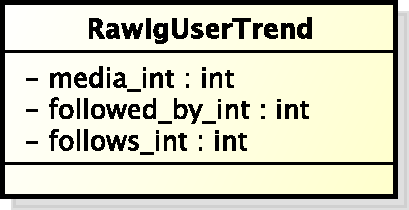
\includegraphics[scale=0.75]{./images/server/classes/db/raw_ig_user_trend.pdf}}
				\caption{Classe - server::db::raw\_data::ig::RawIgUserTrend}
			\end{figure}
			\begin{itemize}
				\item \textbf{Descrizione}: classe che definisce il modello dei dati del trend di un utente Instagram;
				\item \textbf{Utilizzo}: la classe viene utilizzata per memorizzare il numero di media, di followed e follows di una determinata persona. Come per tutti gli oggetti di tipo trend, vengono ricavati i dati fino a 3 giorni prima della creazione dell'oggetto;
				\item \textbf{Classi ereditate}: server::db::raw\_data::AbsRawData
				\item \textbf{Attributi}:
					\begin{itemize}
						\item \textcolor{forestgreen}{\texttt{+ media\_int : int}}
						\begin{description}
							\item \textbf{Descrizione}: numero di media caricati dall'utente su Instagram.
						\end{description}
						\item \textcolor{forestgreen}{\texttt{+ followed\_by\_int : int}}
						\begin{description}
							\item \textbf{Descrizione}: numero di followed dell'utente su Instagram.
						\end{description}
						\item \textcolor{forestgreen}{\texttt{+ follows\_int : int}}
						\begin{description}
							\item \textbf{Descrizione}: numero di following dell'utente su Instagram.
						\end{description}
					\end{itemize}
				\item \textbf{Metodi}: N/A
			\end{itemize}
		% subparagraph server_db_raw_data_ig_rawigusertrend [end]


		\subparagraph{server::db::raw\_data::ig::RawIgHashtag} % (fold)
		\label{subp:server_db_raw_data_ig_rawighashtag}
			\begin{itemize}
				\item \textbf{Descrizione}: classe che definisce il modello dei dati di un hashtag Instagram;
				\item \textbf{Utilizzo}: la classe viene utilizzata per fornire una descrizione minimale dell'hashtag su Instagram. Sebbene tale classe non fornisca metodi o campi dati, risulta molto utile per distinguere un hashtag Instagram da un'altra metrica tramite type checking;
				\item \textbf{Classi ereditate}: server::db::raw\_data::AbsIgRawData
				\item \textbf{Relazioni con altre classi}:
					\begin{itemize}
						\item server::db::raw\_data::ig::RawIgHashtagTrend
						\item server::db::raw\_data::ig::RawIgMedia
					\end{itemize}
				\item \textbf{Attributi}: N/A
				\item \textbf{Metodi}: N/A
			\end{itemize}
		% subparagraph server_db_raw_data_ig_rawighashtag [end]


		\subparagraph{server::db::raw\_data::ig::RawIgHashtagTrend} % (fold)
		\label{subp:server_db_raw_data_ig_rawighashtagtrend}
			\begin{figure}[htbp]
				\centering
				\centerline{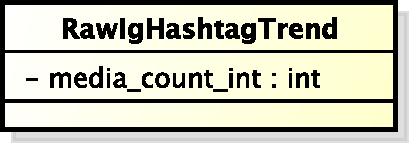
\includegraphics[scale=0.75]{./images/server/classes/db/raw_ig_hashtag_trend.pdf}}
				\caption{Classe - server::db::raw\_data::ig::RawIgHashtagTrend}
			\end{figure}
			\begin{itemize}
				\item \textbf{Descrizione}: classe che definisce il modello dei dati del trend di un hashtag Instagram;
				\item \textbf{Utilizzo}: la classe viene utilizzata per memorizzare il numero di media caricati di un determinato hashtag. Come per tutti gli oggetti di tipo trend, vengono ricavati i dati fino a 3 giorni prima della creazione dell'oggetto;
				\item \textbf{Classi ereditate}: server::db::raw\_data::AbsRawData
				\item \textbf{Attributi}:
					\begin{itemize}
						\item \textcolor{forestgreen}{\texttt{+ media\_count\_int : int}}
						\begin{description}
							\item \textbf{Descrizione}: numero totale di media relativi ad un hashtag su Instagram.
						\end{description}
					\end{itemize}
				\item \textbf{Metodi}: N/A
			\end{itemize}
		% subparagraph server_db_raw_data_ig_rawighashtagtrend [end]


		\subparagraph{server::db::raw\_data::ig::RawIgMedia} % (fold)
		\label{subp:server_db_raw_data_ig_rawigmedia}
			\begin{figure}[htbp]
				\centering
				\centerline{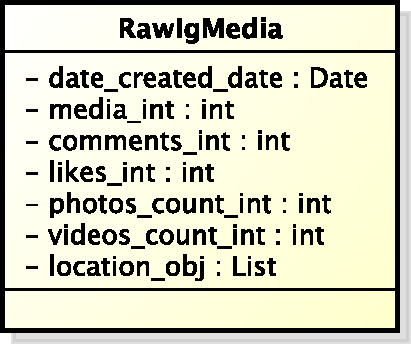
\includegraphics[scale=0.75]{./images/server/classes/db/raw_ig_media.pdf}}
				\caption{Classe - server::db::raw\_data::ig::RawIgMedia}
			\end{figure}
			\begin{itemize}
				\item \textbf{Descrizione}: classe che definisce il modello dei dati di un media relativo ad Instagram;
				\item \textbf{Utilizzo}: la classe viene utilizzata per fornire una descrizione dettagliata del trend dei media relativi ad un utente o un hashtag specifico su Instagram. Come per tutti gli oggetti di tipo trend, vengono ricavati i dati fino a 3 giorni prima della creazione dell'oggetto;
				\item \textbf{Classi ereditate}: server::db::raw\_data::AbsRawData
				\item \textbf{Attributi}:
					\begin{itemize}
						\item \textcolor{forestgreen}{\texttt{+ media\_int : int}}
						\begin{description}
							\item \textbf{Descrizione}: numero di media ricavati.
						\end{description}
						\item \textcolor{forestgreen}{\texttt{+ comments\_int : int}}
						\begin{description}
							\item \textbf{Descrizione}: numero totale dei commenti presenti in tutti i media ricavati.
						\end{description}
						\item \textcolor{forestgreen}{\texttt{+ likes\_int : int}}
						\begin{description}
							\item \textbf{Descrizione}: numero totale dei likes presenti in tutti i media ricavati.
						\end{description}
						\item \textcolor{forestgreen}{\texttt{+ photos\_count\_int : int}}
						\begin{description}
							\item \textbf{Descrizione}: numero totale di media di tipo foto.
						\end{description}
						\item \textcolor{forestgreen}{\texttt{+ videos\_count\_int : int}}
						\begin{description}
							\item \textbf{Descrizione}: numero totale di media di tipo video.
						\end{description}
						\item \textcolor{forestgreen}{\texttt{+ location\_obj : GeoPoint}}
						\begin{description}
							\item \textbf{Descrizione}: localizzazione tramite latitudine e longitudine di un media su Instagram.
						\end{description}
					\end{itemize}
				\item \textbf{Metodi}: N/A
			\end{itemize}
		% subparagraph server_db_raw_data_ig_rawigmedia [end]

\subsubsection{server::db::app\_data} % (fold)
\label{ssub:bdsm_app_server_app_data}


	\begin{figure}[htbp]
		\centering
		\centerline{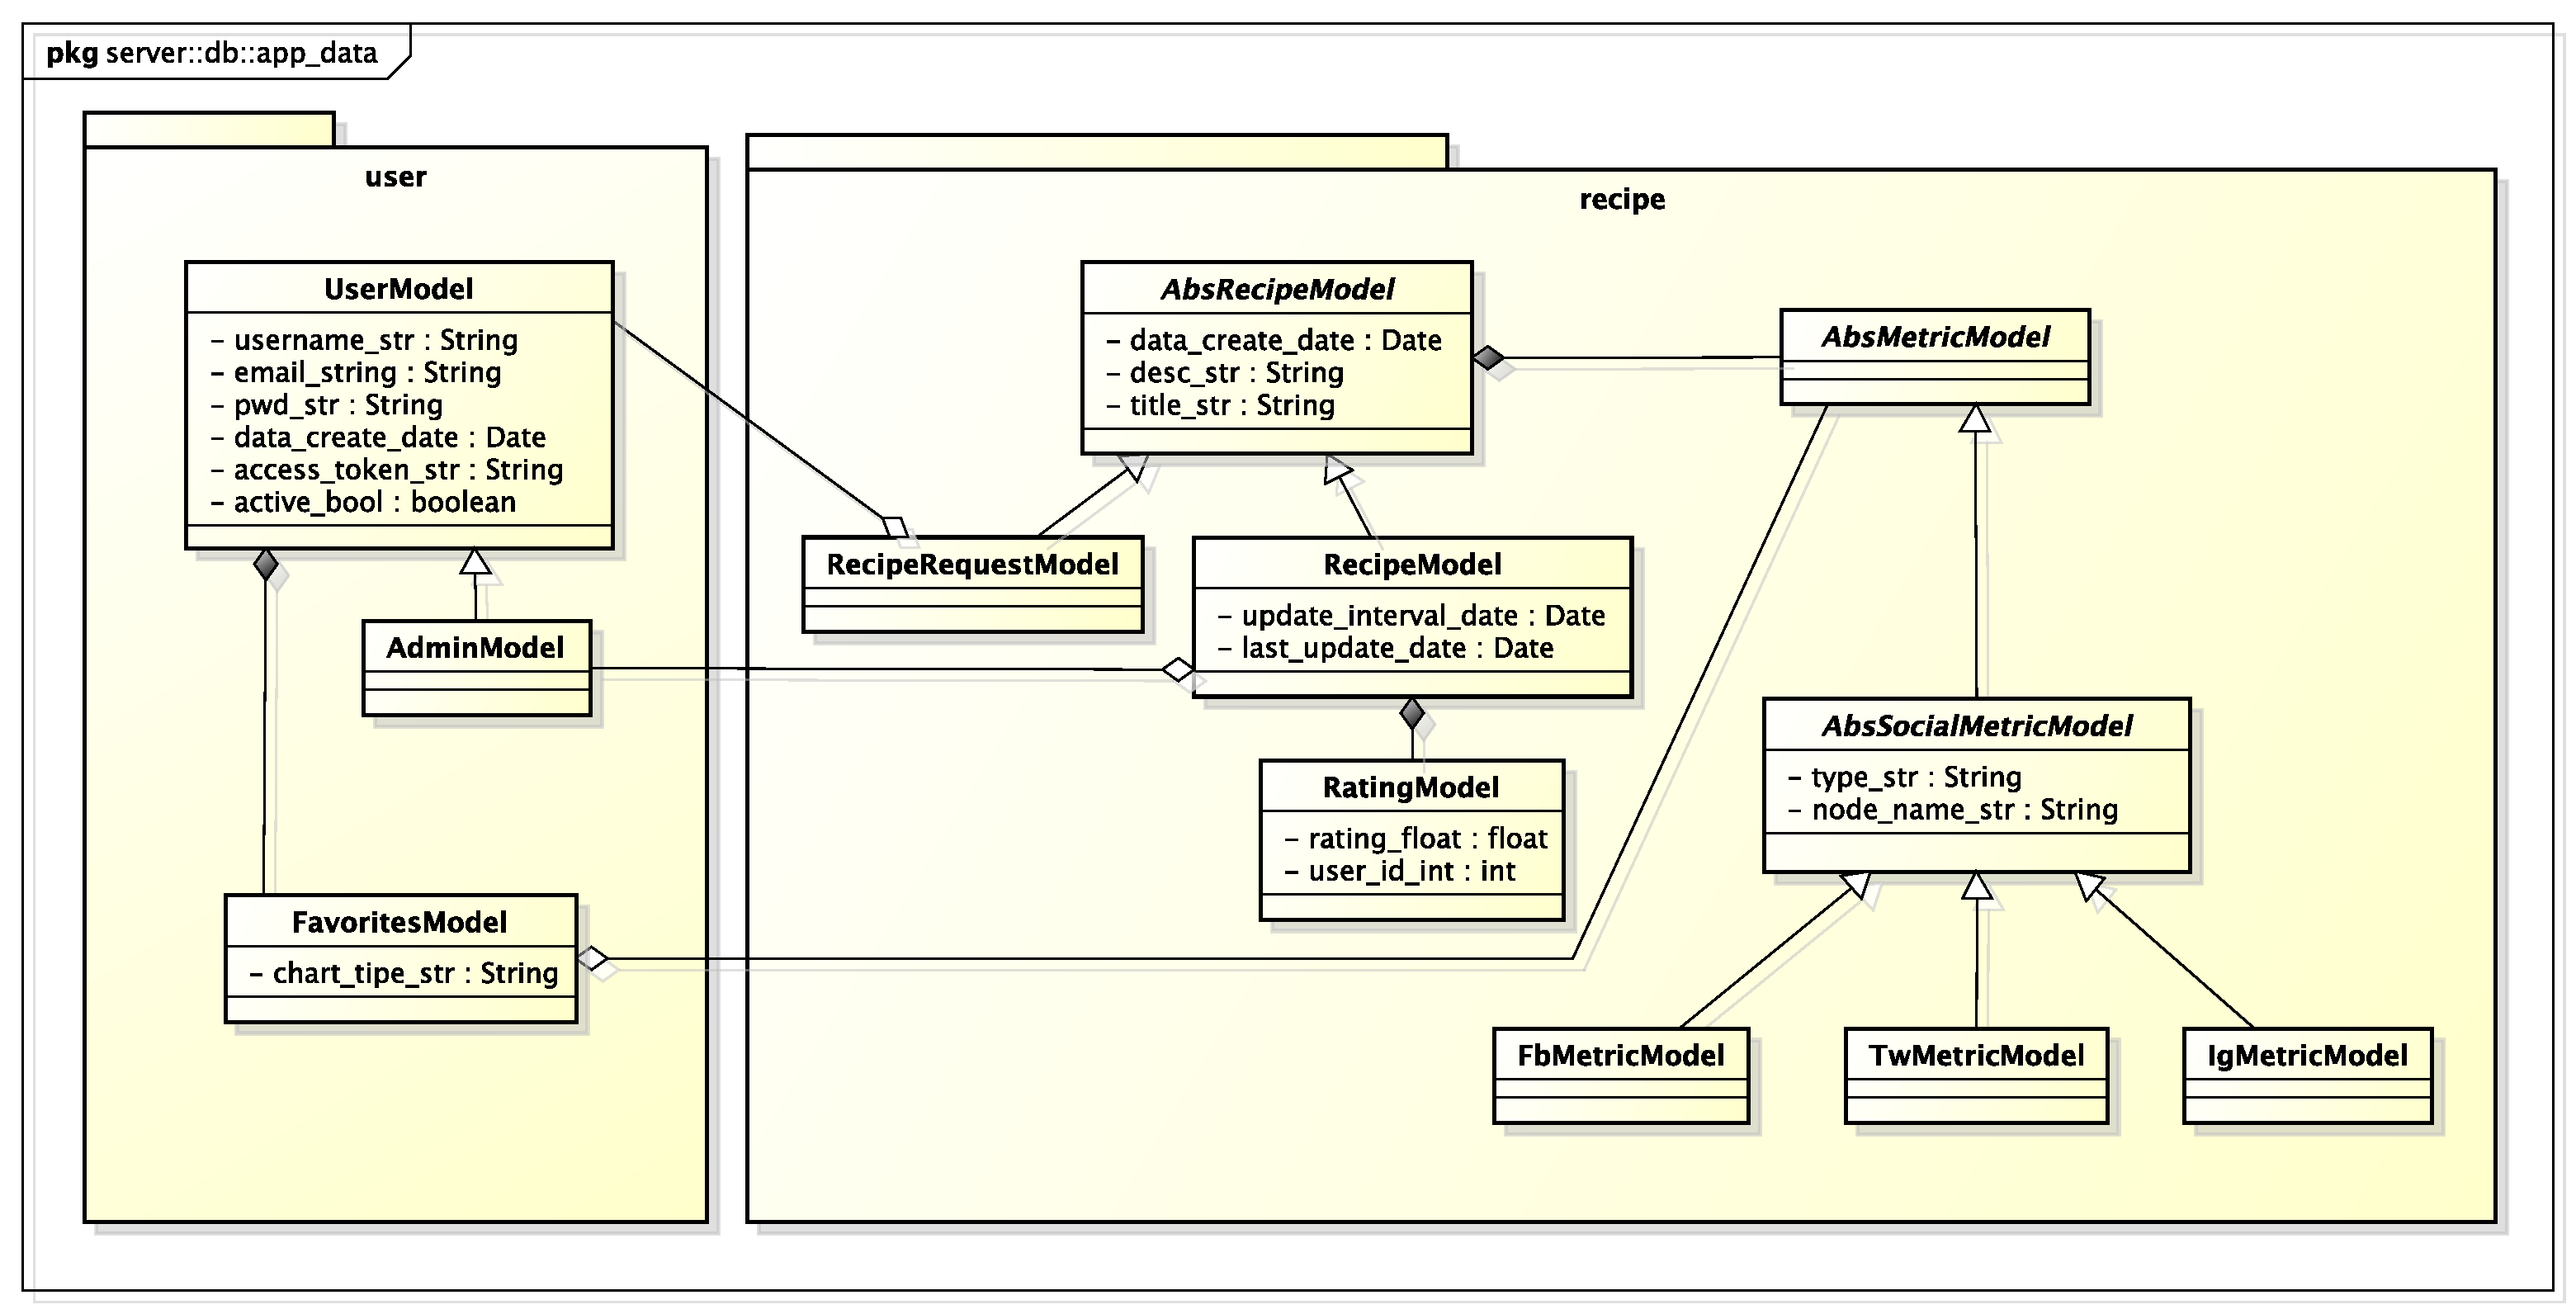
\includegraphics[scale=0.38]{./images/server/app_data.pdf}}
		\caption{Package - server::db::app\_data}
	\end{figure}


	\begin{itemize}
		\item \textbf{Descrizione}: è il package che contiene la definizione dei modelli degli utenti registrati e le loro preferenze. Contiene inoltre il modello delle Recipe che l'amministratore decide di creare;
		\item \textbf{Padre}: server::db
		\item \textbf{Package contenuti}
			\begin{itemize}
				\item server::db::app\_data::user
				\item server::db::app\_data::recipe
			\end{itemize}
	\end{itemize}
	% subsubsection bdsm_app_server_app_data [end]


\subsubsection{server::db::app\_data::user} % (fold)
\label{ssub:bdsm_app_server_app_data_user}

	\begin{itemize}
		\item \textbf{Descrizione}: è il package che contiene la definizione dei modelli degli utenti registrati e le loro preferenze;
		\item \textbf{Padre}: server::db::app\_data
		\item \textbf{Interazione con altri componenti}:
			\begin{itemize}
				\item server::db::app\_data::recipe
			\end{itemize}
	\end{itemize}
	% subsubsection bdsm_app_server_app_data_user [end]


	\paragraph{Classi} % (fold)

		\subparagraph{server::db::app\_data::user::UserModel} % (fold)
		\label{subp:server_db_app_data_user_user_model}
			\begin{figure}[htbp]
				\centering
				\centerline{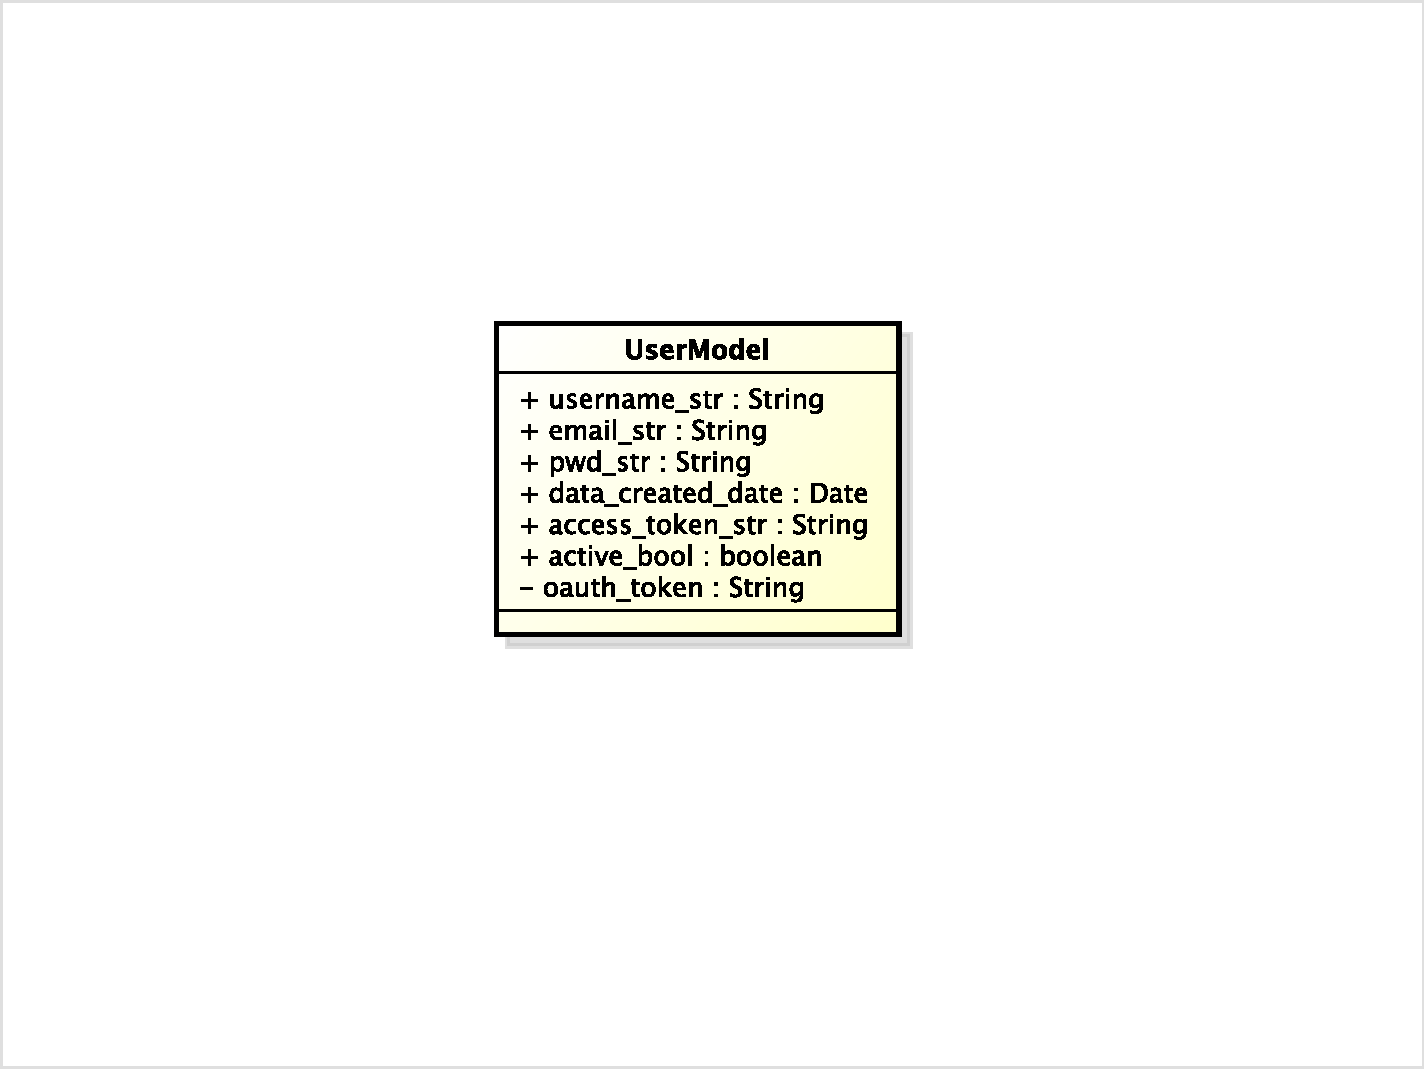
\includegraphics[scale=0.75]{./images/server/classes/db/user_model.pdf}}
				\caption{Classe - server::db::app\_data::user::UserModel}
			\end{figure}
			\begin{itemize}
				\item \textbf{Descrizione}: classe che definisce il modello dei dati degli utenti all'interno della base di dati;
				\item \textbf{Utilizzo}: la classe utilizzata per aggiungere, modificare o eliminare un utente dal database;
				\item \textbf{Relazioni con altre classi}:
					\begin{itemize}
						\item server::db::app\_data::user::FavouritesModel
						\item server::db:::app\_data::user::AdminModel
						\item server::db::app\_data::recipe::RecipeRequestModel
					\end{itemize}
				\item \textbf{Attributi}:
					\begin{itemize}
						\item \textcolor{forestgreen}{\texttt{+ username\_str : String}}
						\begin{description}
							\item \textbf{Descrizione}: lo username dell'utente.
						\end{description}
						\item \textcolor{forestgreen}{\texttt{+ email\_str : String}}
						\begin{description}
							\item \textbf{Descrizione}: l'email dell'utente.
						\end{description}
						\item \textcolor{forestgreen}{\texttt{+ pwd\_str : String}}
						\begin{description}
							\item \textbf{Descrizione}: la password dell'utente.
						\end{description}
						\item \textcolor{forestgreen}{\texttt{+ data\_created\_date : Date}}
						\begin{description}
							\item \textbf{Descrizione}: la data creazione account dell'utente.
						\end{description}
						\item \textcolor{forestgreen}{\texttt{+ access\_token\_str : String}}
						\begin{description}
							\item \textbf{Descrizione}: l'access token utilizzato per i servizi REST.
						\end{description}
						\item \textcolor{forestgreen}{\texttt{+ oauth\_token : String}}
						\begin{description}
							\item \textbf{Descrizione}: il token utilizzato per il processo di autenticazione dell'utente.
						\end{description}
						\item \textcolor{forestgreen}{\texttt{+ active\_bool : boolean}}
						\begin{description}
							\item \textbf{Descrizione}: valore che indica se l'utente attivo nel sistema.
						\end{description}
					\end{itemize}
				\item \textbf{Metodi}: N/A
			\end{itemize}
		% subparagraph server_db_app_data_user_user_model [end]


		\subparagraph{server::db::app\_data::user::AdminModel} % (fold)
		\label{subp:server_db_app_data_user_admin_model}
			\begin{itemize}
				\item \textbf{Descrizione}: classe che definisce il modello dei dati degli utenti amministratori all'interno della base di dati;
				\item \textbf{Utilizzo}: la classe specializza l'utente amministratore. Viene utilizzata esclusivamente per distinguere un amministratore da un utente normale tramite type checking;
				\item \textbf{Classi ereditate}: server::db::app\_data::user::UserModel;
				\item \textbf{Relazioni con altre classi}:
					\begin{itemize}
						\item server::db::app\_data::recipe::RecipeModel
					\end{itemize}
				\item \textbf{Attributi}: N/A
				\item \textbf{Metodi}: N/A
			\end{itemize}
		% subparagraph server_db_app_data_user_admin_model [end]


		\subparagraph{server::db::app\_data::user::FavouritesModel} % (fold)
		\label{subp:server_db_app_data_user_favorites}
			\begin{figure}[htbp]
				\centering
				\centerline{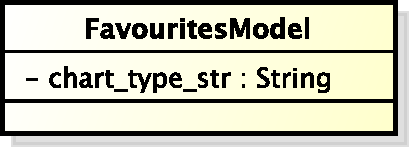
\includegraphics[scale=0.75]{./images/server/classes/db/favourites_model.pdf}}
				\caption{Classe - server::db::app\_data::user::FavouritesModel}
			\end{figure}
			\begin{itemize}
				\item \textbf{Descrizione}: classe che definisce il modello dei dati relativo ai preferiti dell'utente;
				\item \textbf{Utilizzo}: la classe viene utilizzata per memorizzare e ricavare le View preferite relative ad un utente.
				\item \textbf{Relazioni con altre classi}:
					\begin{itemize}
						\item server::db::app\_data::recipe::AbsMetricModel
					\end{itemize}
				\item \textbf{Attributi}:
					\begin{itemize}
						\item \textcolor{forestgreen}{\texttt{chart\_type\_str : String}}
						\begin{description}
							\item \textbf{Descrizione}: tipo di grafico scelto dall'utente e salvato nei preferiti.
						\end{description}
					\end{itemize}
				\item \textbf{Metodi}: N/A
			\end{itemize}
		% subparagraph server_db_app_data_user_favorites [end]


\subsubsection{server::db::app\_data::recipe} % (fold)
\label{ssub:bdsm_app_server_app_data_recipe}

	\begin{itemize}
		\item \textbf{Descrizione}: è il package che contiene la definizione dei modelli delle Recipe che l'amministratore decide di creare;
		\item \textbf{Padre}: server::db::app\_data
		\item \textbf{Interazione con altri componenti}:
			\begin{itemize}
				\item server::db::app\_data::user
			\end{itemize}
	\end{itemize}
	% subsubsection bdsm_app_server_app_data_recipe [end]


	\paragraph{Classi} % (fold)

		\subparagraph{server::db::app\_data::recipe::AbsRecipeModel} % (fold)
		\label{subp:server_db_app_data_recipe_absrecipemodel}
			\begin{figure}[htbp]
				\centering
				\centerline{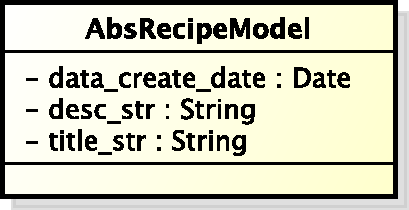
\includegraphics[scale=0.75]{./images/server/classes/db/abs_recipe_model.pdf}}
				\caption{Classe - server::db::app\_data::recipe::AbsRecipeModel}
			\end{figure}
			\begin{itemize}
				\item \textbf{Descrizione}: classe astratta che rappresenta un modello comune per Recipe e richiesta di aggiunta Recipe;
				\item \textbf{Utilizzo}: la classe mantiene l'estensibilità per eventuali nuovi tipi di Recipe;
				\item \textbf{Relazioni con altre classi}:
					\begin{itemize}
						\item server::db::app\_data::recipe::RecipeModel
						\item server::db::app\_data::recipe::RecipeRequestModel
						\item server::db::app\_data::recipe::AbsMetricModel
					\end{itemize}
				\item \textbf{Attributi}:
					\begin{itemize}
						\item \textcolor{forestgreen}{\texttt{data\_create\_date : Date}}
						\begin{description}
							\item \textbf{Descrizione}: data di creazione della Recipe.
						\end{description}
						\item \textcolor{forestgreen}{\texttt{desc\_str : String}}
						\begin{description}
							\item \textbf{Descrizione}: descrizione dettagliata dell Recipe.
						\end{description}
						\item \textcolor{forestgreen}{\texttt{title\_str : String}}
						\begin{description}
							\item \textbf{Descrizione}: titolo della Recipe.
						\end{description}
					\end{itemize}
				\item \textbf{Metodi}: N/A
			\end{itemize}
		% subparagraph server_db_app_data_recipe_absrecipemodel [end]


		\subparagraph{server::db::app\_data::recipe::RecipeRequestModel} % (fold)
		\label{subp:server_db_app_data_recipe_reciperequestmodel}
			\begin{itemize}
				\item \textbf{Descrizione}: classe che definisce il modello dei dati per la richiesta di aggiunta Recipe;
				\item \textbf{Utilizzo}: la classe specializza la richiesta identificandone l'utente tramite il rapporto parent-child delle classi di Google Datastore;
				\item \textbf{Classi ereditate}: server::db::app\_data::recipe::AbsRecipeModel
				\item \textbf{Attributi}: N/A
				\item \textbf{Metodi}: N/A
			\end{itemize}
		% subparagraph server_db_app_data_recipe_reciperequestmodel [end]


		\subparagraph{server::db::app\_data::recipe::RecipeModel} % (fold)
		\label{subp:server_db_app_data_recipe_recipemodel}
			\begin{figure}[htbp]
				\centering
				\centerline{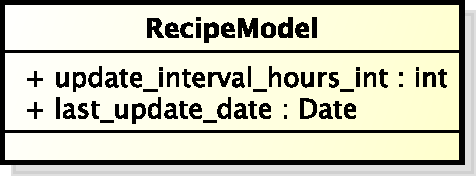
\includegraphics[scale=0.75]{./images/server/classes/db/recipe_model.pdf}}
				\caption{Classe - server::db::app\_data::recipe::RecipeModel}
			\end{figure}
			\begin{itemize}
				\item \textbf{Descrizione}: classe che definisce il modello dei dati relativo ad una Recipe;
				\item \textbf{Utilizzo}: la classe specializza la ricetta. Vengono forniti i campi dati per il possibile incremento temporale dei dati;
				\item \textbf{Classi ereditate}: server::db::app\_data::recipe::AbsRecipeModel
				\item \textbf{Relazioni con altre classi}:
					\begin{itemize}
						\item server::db::app\_data::recipe::RatingModel
					\end{itemize}
				\item \textbf{Attributi}:
					\begin{itemize}
						\item \textcolor{forestgreen}{\texttt{+ update\_interval\_hours\_int : int}}
						\begin{description}
							\item \textbf{Descrizione}: intervallo di tempo per la schedulazione dell'update della Recipe.
						\end{description}
						\item \textcolor{forestgreen}{\texttt{+ last\_update\_date : Date}}
						\begin{description}
							\item \textbf{Descrizione}: data dell'ultimo processo di update Recipe.
						\end{description}
					\end{itemize}
				\item \textbf{Metodi}: N/A
			\end{itemize}
		% subparagraph server_db_app_data_recipe_recipemodel [end]

		\subparagraph{server::db::app\_data::recipe::RatingModel} % (fold)
		\label{subp:server_db_app_data_recipe_recipemodel}
			\begin{figure}[htbp]
				\centering
				\centerline{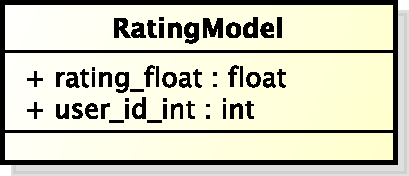
\includegraphics[scale=0.75]{./images/server/classes/db/rating_model.pdf}}
				\caption{Classe - server::db::app\_data::recipe::RatingModel}
			\end{figure}
			\begin{itemize}
				\item \textbf{Descrizione}: classe che rappresenta il modello del rating di una Recipe;
				\item \textbf{Utilizzo}: viene utilizzata per risalire al voto di ogni utente per una determinata Recipe;
				\item \textbf{Attributi}:
					\begin{itemize}
						\item \textcolor{forestgreen}{\texttt{+ rating\_float : float}}
						\begin{description}
							\item \textbf{Descrizione}: punteggio gradimento relativo alla Recipe.
						\end{description}
						\item \textcolor{forestgreen}{\texttt{+ user\_id\_int : int}}
					\end{itemize}
					\begin{description}
							\item \textbf{Descrizione}: identificativo dell'utente votante.
						\end{description}
				\item \textbf{Metodi}: N/A
			\end{itemize}
		% subparagraph server_db_app_data_recipe_recipemodel [end]


		\subparagraph{server::db::app\_data::recipe::AbsMetricModel} % (fold)
		\label{subp:server_db_app_data_recipe_absmetricmodel}
			\begin{itemize}
				\item \textbf{Descrizione}: classe che definisce il modello dei dati di una metrica contenuta in una Ricetta;
				\item \textbf{Utilizzo}: la classe rappresenta il modello dei dati di una metrica generale;
				\item \textbf{Relazioni con altre classi}:
					\begin{itemize}
						\item server::db::app\_data::recipe::AbsSocialMetricModel
					\end{itemize}
				\item \textbf{Attributi}: N/A
				\item \textbf{Metodi}: N/A
			\end{itemize}
		% subparagraph server_db_app_data_recipe_absmetricmodel [end]


		\subparagraph{server::db::app\_data::recipe::AbsSocialMetricModel} % (fold)
		\label{subp:server_db_app_data_recipe_abssocialmetricmodel}
			\begin{figure}[htbp]
				\centering
				\centerline{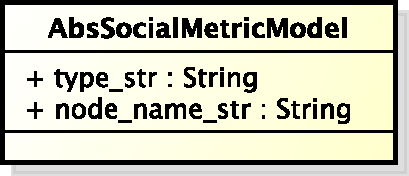
\includegraphics[scale=0.75]{./images/server/classes/db/abs_social_metric_model.pdf}}
				\caption{Classe - server::db::app\_data::recipe::AbsSocialMetricModel}
			\end{figure}
			\begin{itemize}
				\item \textbf{Descrizione}: classe che definisce il modello dei dati delle metriche relative ai social media;
				\item \textbf{Utilizzo}: la classe rappresenta il modello di una metrica relativa ad un social network fornendo il tipo di metrica e il suo identificativo;
				\item \textbf{Classi ereditate}: server::db::app\_data::recipe::AbsMetricModel
				\item \textbf{Relazioni con altre classi}:
					\begin{itemize}
						\item server::db::app\_data::recipe::FbMetricModel
						\item server::db::app\_data::recipe::IgMetricModel
						\item server::db::app\_data::recipe::TwMetricModel
					\end{itemize}
				\item \textbf{Attributi}:
					\begin{itemize}
						\item \textcolor{forestgreen}{\texttt{+ type\_str : String}}
						\begin{description}
							\item \textbf{Descrizione}: tipo della metrica (pagina, evento, hashtag).
						\end{description}
						\item \textcolor{forestgreen}{\texttt{+ node\_name\_str : String}}
						\begin{description}
							\item \textbf{Descrizione}: nome identificativo della metrica.
						\end{description}
					\end{itemize}
				\item \textbf{Metodi}: N/A
			\end{itemize}
		% subparagraph server_db_app_data_recipe_abssocialmetricmodel [end]


		\subparagraph{server::db::app\_data::recipe::FbMetricModel} % (fold)
		\label{subp:server_db_app_data_recipe_fbmetricmodel}
			\begin{itemize}
				\item \textbf{Descrizione}: classe che definisce il modello dei dati delle metriche relative a Facebook;
				\item \textbf{Utilizzo}: viene utilizzata esclusivamente per offrire una distinzione di tipo per le metriche relative a Facebook rispetto ai restanti social network;
				\item \textbf{Classi ereditate}: server::db::app\_data::recipe::AbsSocialMetricModel;
				\item \textbf{Attributi}: N/A
				\item \textbf{Metodi}: N/A
			\end{itemize}
		% subparagraph server_db_app_data_recipe_fbmetricmodel [end]


		\subparagraph{server::db::app\_data::recipe::IgMetricModel} % (fold)
		\label{subp:server_db_app_data_recipe_igmetricmodel}
			\begin{itemize}
				\item \textbf{Descrizione}: classe che definisce il modello dei dati delle metriche relative a Instagram;
				\item \textbf{Utilizzo}: viene utilizzata esclusivamente per offrire una distinzione di tipo per le metriche relative a Instagram rispetto ai restanti social network;
				\item \textbf{Classi ereditate}: server::db::app\_data::recipe::AbsSocialMetricModel;
				\item \textbf{Attributi}: N/A
				\item \textbf{Metodi}: N/A
			\end{itemize}
		% subparagraph server_db_app_data_recipe_igmetricmodel [end]


		\subparagraph{server::db::app\_data::recipe::TwMetricModel} % (fold)
		\label{subp:server_db_app_data_recipe_twmetricmodel}
			\begin{itemize}
				\item \textbf{Descrizione}: classe che definisce il modello dei dati delle metriche relative a Twitter;
				\item \textbf{Utilizzo}: viene utilizzata esclusivamente per offrire una distinzione di tipo per le metriche relative a Twitter rispetto ai restanti social network;
				\item \textbf{Classi ereditate}: server::db::app\_data::recipe::AbsSocialMetricModel;
				\item \textbf{Attributi}: N/A
				\item \textbf{Metodi}: N/A
			\end{itemize}
		% subparagraph server_db_app_data_recipe_twmetricmodel [end]
